\documentclass{article}
\usepackage[utf8]{inputenc}
\usepackage{graphicx}
\usepackage{float}
\usepackage[skip=2pt]{caption}
\usepackage{geometry}
\usepackage{subcaption}
\usepackage{amssymb}
\usepackage{amsmath}
\usepackage{booktabs}
\usepackage{hyperref}
\usepackage{array}
\usepackage{tabularx}
\usepackage[table]{xcolor}
\usepackage{natbib}
\geometry{margin=1in}

\title{\textbf{Newsvendor Problem: Theory and Applications}}
\author{Group 8 \\ \\Thijs van Dijkman, Xiaoyang Liu, Chinechem Okere, Michał Śliwiński, Anthony Vári}
\date{}

\begin{document}

\maketitle
\bigskip

\section*{Task 1: Introduction}
\noindent The Newsvendor Problem (NVP) addresses a classic model used in inventory management that helps determine how much stock a decision-maker, facing uncertain demand, should order. It is most relevant for perishable products or seasonal goods because their value decreases over time, meaning that an overstocking results in financial loss. The purpose of the model is to determine the optimal order quantity that takes the risk of having too little inventory and the risk of ordering too much and balances them out to maximize expected profit.

The NVP provides a solid foundation for solving real-world decision-making problems when faced with uncertainty. In practice, companies often face the challenge of having to interpret varying historical demand data and derive feasible stocking decisions from them. For example, a clothing store might rely on past sales to forecast demand for seasonal items such as winter jackets. The model allows them to use these forecasts to determine an optimal order quantity that balances the risk of overstocking with the risk of missing potential sales. This trade-off also applies to services. Mobile service providers such as Vodafone face similar trade-offs when designing their bundles. An order quantity that is too high can lead to unused resources, while one that is too low risks customer dissatisfaction. What makes the NVP especially useful here is its mathematical convenience. When the demand distribution is known, the optimal order quantity corresponds to a specific quantile of that distribution, which can be computed using Python. The ability to go from probabilistic modeling to precise numerical solutions is what makes the NVP a powerful tool in data science.

However, the NVP has its limitations and challenges. A big challenge in real-life applications of the Newsvendor Problem is the difficulty in demand estimation. Accurate modeling of demand distribution is often hard due to limited data, seasonal trends, or other various outside factors. For instance, the COVID-19 pandemic massively affected consumer behavior, making historical data much less reliable. Moreover, real costs of under- or over-stocking are not always fully shown by the cost and price parameters. To tackle this, we introduce methods such as parametric estimation (for example fitting normal or Poisson distributions to demand data) and nonparametric, quantile-based estimators. These allow decision-makers to do their job without having to rely solely on strict assumptions. Machine learning methods can improve forecasting of demand and simulations like the Monte Carlo one methods can help evaluate how different order quantities perform in different scenarios. 

These methods extend beyond inventory settings. For example, in healthcare logistics, quantile-based models are used to manage uncertain demand for critical resources such as hospital beds or blood products. \cite{shen2024} use a data-driven newsvendor framework to balance elective and emergency patient admissions under an uncertain hospital capacity. Their approach avoids assuming a known demand distribution and instead uses the historical data to estimate the optimal service level. This shows how quantile-based decision rules remain effective even when faced with unstable, high-stakes demand.
Similarly, \cite{patra2021} use a two-period newsvendor model in disaster relief logistics. They optimize how much aid to station before a disaster and how much to send afterward, using Bayesian updates to reflect real-time information. This expansion shows how newsvendor-based reasoning applies in emergency situations, where the cost of over- or under-supplying is both financial and human.
In this project, we will explore its relevance in a more everyday setting: a bakery chain from Vilnius. This project builds on the classical NVP and applies its logic and methods to a practical case study involving the day-to-day operations of the business. The business faces a previously covered tradeoff: bake too little and miss out on potential profit, or bake too much and either create waste or lose money on clearance sales. There are also additional factors such as demand changes for different days of the week, store-specific characteristics, and external factors such as the COVID-19 pandemic. Our goal is to estimate optimal production quantities that maximize expected profit using historical demand data.

When working on the Vilnius bakery problem, we will use both parametric and nonparametric estimation methods introduced in the course. In Task 2, we will revise the classical Newsvendor profit function to take into account the clearance price and shipping cost, making the model more applicable in the context of the bakery. We will analyze how increasing the shipping cost \( c_S \) will affect the optimal order quantity and the expected profit.

In Task 3, we will perform a Monte Carlo simulation study to compare the performance of the parametric and nonparametric estimators across different service levels and sample sizes. We will focus on the Root Mean Squared Error (RMSE), Profit Loss Ratio (PLR), and Service Level (SL). The goal is to confirm the assumption that, under correctly fitted distributions, the parametric method outperforms the nonparametric one in both accuracy and profit outcomes. However, we observe that the nonparametric estimator will remain useful when the true demand distribution is uncertain.

In Task 4, we will test how the modeling error of the demand distribution impacts the estimate of order quantity. We will generate demand data from non-normal distributions (Poisson and Exponential) and then fit a normal distribution to each sample. For every value $\tau$ we had, we estimate the value of $\hat{Q}$ using the fitted normal distribution and compare it to the true quantile $Q^*$ of the actual distribution by calculating their absolute error. To avoid any uncertainty caused by noise or randomness, we will run the simulation 1000 times for different values of $\tau$ and various sample sizes to evaluate how the misspecification error differs across quantiles and distributions when assuming a normal model incorrectly.

So far, our findings show that extending the classical Newsvendor model to include the shipping costs and clearance prices results in more realistic stocking recommendations. When the model is correctly specified, the parametric estimator outperforms the non-parametric one both in RMSE and PLR, but the latter is more robust when facing uncertainty or model misspecification. These findings suggest a hybrid approach: Use parametric models when the distribution is known and nonparametric when the data and knowledge are uncertain.

The following sections build on this. Section 2.2 elaborates on the theoretical aspects of the Newsvendor Problem and its methods. Section 2.3 applies these models to a real-world problem and evaluates the Vilnius bakery dataset. Finally, Section 2.4 reflects on the strengths and limitations of the approaches we used and discusses potential improvements and further research.

\section*{Task 2: Theoretical Questions}
\subsubsection*{\boldmath a) Justification for $p_L < c + c_S$}
\noindent
When the \emph{Vilnius} bakery has unsold surplus product, it has a deal with a local feed mill that purchases the surplus at a lower price, denoted as $p_L$. 
In practice, this price should be lower than the sum of the shipping costs and the production costs denoted as $c + c_S$, because otherwise it would create an incentive for the bakery to overproduce on purpose in order to generate more profit when trading with the animal feed producer. In the situation where $p_L \geq c + c_S$, the business model would deem the business model of a bakery entirely unoptimal. This is because distributing the product between customers would generate less profit or the same amount of profit as simply selling it to the feed producer. The inequality $p_L < c + c_S$ ensures that shipping leftovers

This ensures that $p_L < c + c_S$ keeps customer sales profitable while allowing the feed mill to function as a mean to minimize losses. 

\subsubsection*{\boldmath b) Adding $p_L$ and $c_S$ to the profit function}
\noindent 
To incorporate the $p_L$ %(clearance price) 
and the $c_S$, %(shipping cost)
 we will modify the classical profit function:

\[
\Pi(Q, Y; c, p) = p \cdot \min\{Q, Y\} - c \cdot Q
\]
\noindent
If we now include clearance sales, where we have $Q - Y$ unsold units, if $Q > Y$. Then these are sold at price $p_L$, and the costs of shipping them are $c_S$ per unit, then our profit function becomes:

\[
\Pi(Q, Y; c, p, p_L, c_S) = p \cdot \min\{Q, Y\} + (p_L - c_S) \cdot (Q - Y)^+ - c \cdot Q,
\]
\noindent
where $(Q - Y)^+ = \max(Q - Y, 0)$ denotes the number of surplus units.


\noindent
\\We want to simplify the form to match:

\[
\Pi(Q, Y; \tilde{c}, \tilde{p}) = \tilde{p} \cdot \min\{Q, Y\} - \tilde{c} \cdot Q,
\]
\noindent
where $\tilde{p}$ and $\tilde{c}$ represent adjusted effective values. In this setup, we define:

\[
\tilde{p} = p, \quad \tilde{c} = c - (p_L - c_S) \cdot \mathbb{P}(Q > Y).
\]

\noindent
The term $\tilde{c}$ is the effective cost per unit, reduced by the expected value recovered from the sale of surplus goods to the feed mill. It is important to note that this simplification is only an approximate and depends on the expected surplus, which differs depending on the distribution of $Y$. This expression simplifies the analysis, but for best accuracy it is better to use the original function that has explicit terms representing the surplus.


\subsubsection*{c) Optimal Order Quantity with adjusted costs}
\noindent 
With a known demand distribution with (CDF) $F_Y$, and effective cost and price values $\tilde{c}$ and $\tilde{p}$, the optimal order quantity is given by the critical fractile formula:

\[
Q^*(F_Y; \tilde{c}, \tilde{p}) = F_Y^{-1} \left( \frac{\tilde{p} - \tilde{c}}{\tilde{p}} \right).
\]

\noindent
Where, as previously defined in section \textbf{b)}, $\tilde{p} = p$, and $\tilde{c} = c - (p_L - c_S) \cdot \mathbb{P}(Q > Y)$, the optimal order quantity becomes:

\[
Q^* = F_Y^{-1} \left( \frac{p - \tilde{c}}{p} \right).
\]
\noindent
Note that $\tilde{c}$ depends on the probability of having surplus, which itself depends on $Q$. This equation is technically implicit, but it can be used directly when $\tilde{c}$ is treated as fixed.


\subsubsection*{\boldmath d) Impact of Shipping Cost on $Q*$ and Expected Profit}

We fix the parameters $c = 1$, $p = 1.5$, $p_L = 0.15$, and assume that the demand follows a normal distribution $Y \sim \mathcal{N}(110, 10^2)$. Our objective is to study how changes in the shipping cost $c_S$ affect the optimal order quantity $Q^*$ and the expected profit $\mathbb{E}[\Pi(Q, Y)]$. \bigskip

\noindent
For each value of $c_S \in [0, 0.5]$, we calculate the adjusted cost:
\[
\tilde{c} = c - (p_L - c_S) \cdot \mathbb{P}(Q > Y),
\]
and then use the critical formula to determine the optimal order quantity.
\[
Q^* = F_Y^{-1} \left( \frac{p - \tilde{c}}{p} \right),
\]

Next, we estimate the expected profit which results from ordering a quantity $Q^*$. In an ideal case where all units are sold, the profit would simply be $(p - c) \cdot Q$,
since each unit generates $(p - c)$ in profit and $Q$ units are ordered.

However, since demand is uncertain, we must adjust this for the possibility of overstocking. To do so, we subtract an integral term that estimates the expected cost of ordering too much units and get this expression for expected profit:
\[
\mathbb{E}[\Pi(Q, Y)] = (p - c) \cdot Q - p \cdot \int_{-\infty}^{Q} F_Y(y) \, dy,
\]
where $F_Y(y)$ is the CDF of the demand.

The integral reflects the accumulated probability of lower demand values and captures how often the order quantity $Q$ is larger than the actual demand. This expression gives us a more realistic estimate of profit because it factors in the cost of excess inventory. These approximations are done using Python.

\bigskip \bigskip

The figure below illustrates how $Q^*$ and expected profit change as $c_S$ increases:

\begin{itemize}
    \item As $c_S$ increases, the marginal value of selling surplus goods decreases, and, consequently, the optimal order quantity ($Q^*$) steadily decreases. This reflects a more conservative stocking strategy to avoid excess.
    
    \item The expected profit remains relatively stable for small $c_S$ values but declines more rapidly as $c_S$ approaches 0.5. This indicates that at one point excessive shipping costs start outweighing the benefits of clearance sales.
\end{itemize}

\begin{figure}[H]
    \centering
    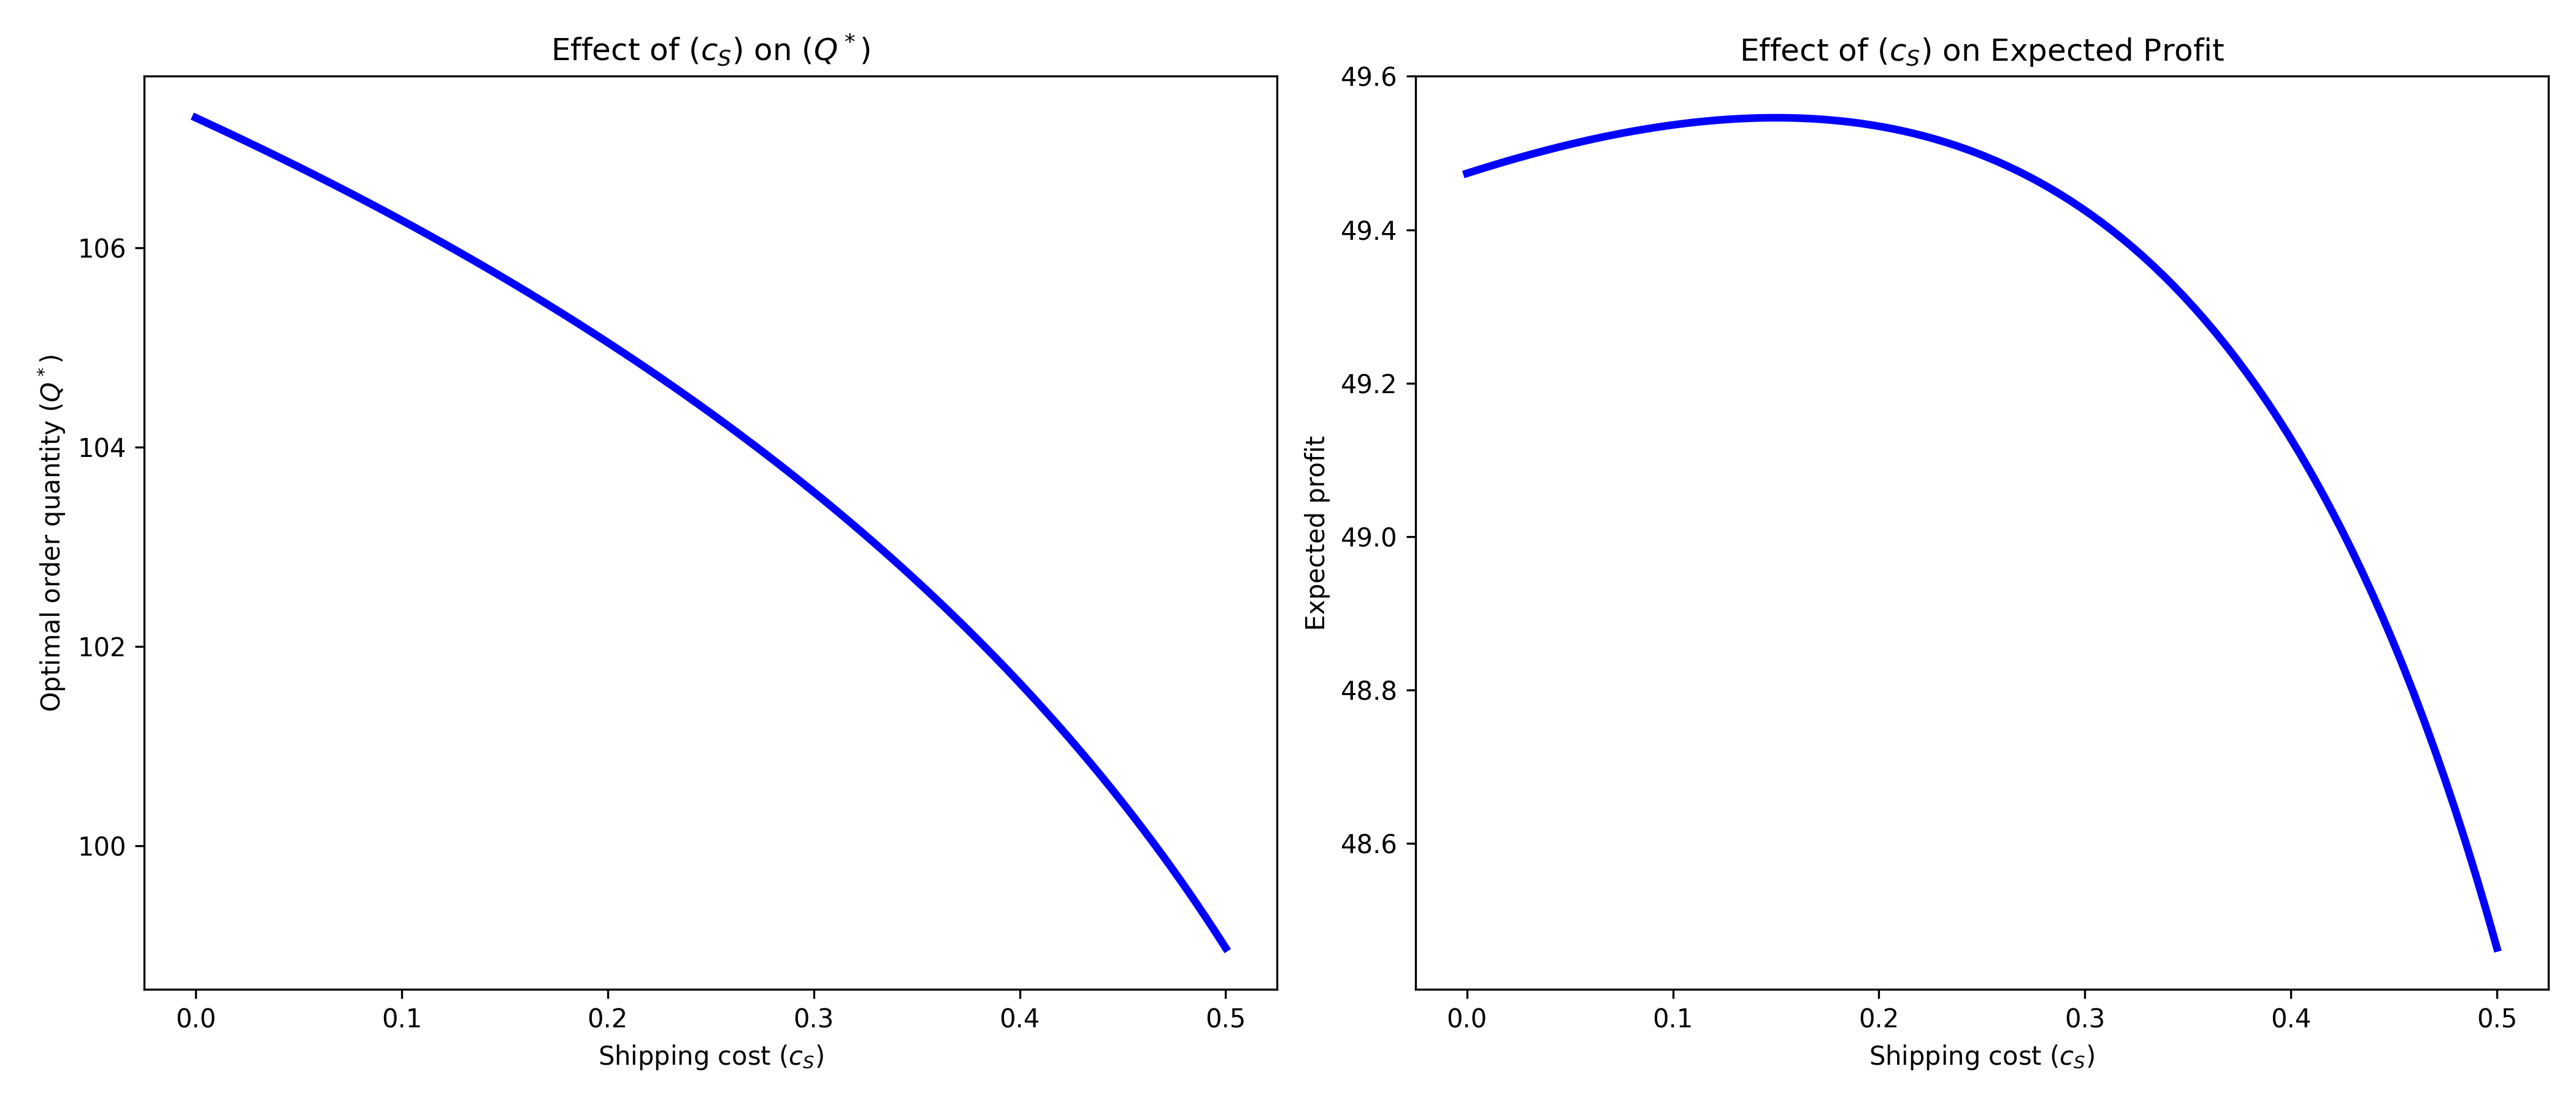
\includegraphics[width=1.00\textwidth]{figures/task2plot.png}
    \caption{Effect of shipping cost $c_S$ on optimal order quantity and expected profit}
\end{figure}


\section*{Task 3: Newsvendor Model Analysis}
The newsvendor model is applicable in this case as the bakery faces uncertain demand, while selling same-day perishable goods. This creates a trade-off between the risks of lost sales (understocking) and spoilage (overstocking). Given demand variability and unknown true distribution, optimal order quantity must be estimated.

One method assumes a parametric distribution \( f(x; \theta) \), e.g., normal, with parameters estimated from historical data. Bootstrap samples \( X^* \sim f(x; \theta) \) are then generated.

Alternatively, the nonparametric approach resamples directly from the empirical distribution function (EDF), defined as:
\[
F(y) = \frac{1}{n} \sum_{i=1}^{n} H(y - y_i)
\]
where \( H(u) \) is the unit step function (1 if \( u \geq 0 \), 0 otherwise).

\paragraph{Root-Mean-Square Error (RMSE)} 
\[
\text{RMSE} = \sqrt{ \frac{1}{M} \sum_{i=1}^{n} (P_i - O_i)^2 }
\]
This measures the average magnitude of prediction error, where \( P_i \) are predicted and \( O_i \) observed values (see \cite{willmott2005} for discussion on the advantages of RMSE over MAE)

\paragraph{Empirical Price Loss Ratio (PLR)} 
\[
\text{PLR}_n^k(\tau) = \frac{1}{M} \sum_{j=1}^M \left| \frac{R(Q^*; \tau) - R(\hat{Q}_{n,j}^k(\tau); \tau)}{R(Q^*; \tau)} \right|
\]
PLR compares profit between the estimated order and optimal order, normalized by the optimal expected profit.

\paragraph{Empirical Service Level (SL)} 
\[
\text{SL}_n^k(\tau) = \frac{1}{M} \sum_{j=1}^M I\left\{ \hat{Q}_{n,j}^k(\tau) \geq Y_j \right\}
\]
This measures the percentage of simulations in which the estimated order quantity covers the actual demand.

\begin{table}[H]
\centering
\caption{RMSE$^P_n(\tau)$}
\label{tab:rmse_p}
\renewcommand{\arraystretch}{1.2}
\begin{tabular}{|c|c|c|c|c|c|c|c|c|c|c|}
\hline
$n \backslash \tau$ & 0.01 & 0.05 & 0.1 & 0.3 & 0.5 & 0.7 & 0.9 & 0.95 & 0.99 \\
\hline
10  & 6.212218 & 4.899544 & 4.472625 & 3.344246 & 3.24019 & 3.36837 & 4.37373 & 4.882186 & 6.219007 \\
50  & 2.76907  & 2.18982  & 1.850608 & 1.481755 & 1.465837 & 1.494265 & 1.899898 & 2.154807 & 2.736072 \\
100 & 1.905263 & 1.537951 & 1.336774 & 1.080217 & 1.014662 & 1.083056 & 1.33693  & 1.563087 & 1.881672 \\
200 & 1.354468 & 1.044762 & 0.959343 & 0.771061 & 0.692413 & 0.741837 & 0.947804 & 1.057911 & 1.368015 \\
\hline
\end{tabular}
\end{table}

\begin{table}[H]
\centering
\caption{RMSE$^{NP}_n(\tau)$}
\label{tab:rmse_np}
\renewcommand{\arraystretch}{1.2}
\begin{tabular}{|c|c|c|c|c|c|c|c|c|c|c|}
\hline
$n \backslash \tau$ & 0.01 & 0.05 & 0.1 & 0.3 & 0.5 & 0.7 & 0.9 & 0.95 & 0.99 \\
\hline
10  & 9.71554  & 5.972408 & 6.361219 & 4.463283 & 4.097794 & 4.205848 & 5.503998 & 5.828964 & 9.744622 \\
50  & 4.806933 & 2.854802 & 2.551798 & 1.861882 & 1.826107 & 1.856143 & 2.492242 & 2.93719  & 4.622108 \\
100 & 4.777829 & 2.229433 & 1.717099 & 1.318972 & 1.273402 & 1.306101 & 1.71034  & 2.109493 & 3.473043 \\
200 & 2.989058 & 1.466918 & 1.240388 & 0.952299 & 0.883723 & 0.925386 & 1.183279 & 1.448877 & 2.587599 \\
\hline
\end{tabular}
\end{table}


\begin{table}[H]
\centering
\caption{ $\frac{\text{RMSE}^{NP}_n(\tau)}{\text{RMSE}^{P}_n(\tau)}$ }
\label{tab:rmse_ratio}
\renewcommand{\arraystretch}{1.2}
\begin{tabular}{|c|c|c|c|c|c|c|c|c|c|c|}
\hline
$n \backslash \tau$ & 0.01 & 0.05 & 0.1 & 0.3 & 0.5 & 0.7 & 0.9 & 0.95 & 0.99 \\
\hline
10  & 1.563941 & 1.218972 & 1.422256 & 1.334616 & 1.264677 & 1.24863  & 1.258422 & 1.193925 & 1.56691  \\
50  & 1.735938 & 1.303669 & 1.378897 & 1.256542 & 1.245778 & 1.242178 & 1.311777 & 1.363087 & 1.689322 \\
100 & 2.507701 & 1.449612 & 1.28451  & 1.221025 & 1.255001 & 1.20594  & 1.279303 & 1.349569 & 1.845722 \\
200 & 2.206813 & 1.404069 & 1.292955 & 1.235051 & 1.276296 & 1.247425 & 1.248443 & 1.369565 & 1.891499 \\
\hline
\end{tabular}
\end{table}


As shown in Table~\ref{tab:rmse_p}
and Table~\ref{tab:rmse_np}, the RMSE of the parametric estimator is generally lower than that of the non-parametric estimator. A clearer comparison can be made by calculating the RMSE ratio in Table~\ref{tab:rmse_ratio}, since a lower RMSE indicates a more accurate estimator. Under the assumption of a correctly specified model, the parametric method is more precise.

\begin{table}[H]
\centering
\caption{ $\frac{\text{PLR}^{NP}_n(\tau)}{\text{PLR}^{P}_n(\tau)}$ }
\label{tab:plr_ratio}
\renewcommand{\arraystretch}{1.2}
\begin{tabular}{|c|c|c|c|c|c|c|c|c|c|c|}
\hline
$n \backslash \tau$ & 0.01 & 0.05 & 0.1 & 0.3 & 0.5 & 0.7 & 0.9 & 0.95 & 0.99 \\
\hline
10  & 1.616788 & 1.198526 & 1.455372 & 1.384312 & 1.381471 & 1.392850 & 1.557540 & 1.219940 & 1.931809 \\
50  & 1.706672 & 1.300384 & 1.370660 & 1.268158 & 1.287416 & 1.258040 & 1.383551 & 1.361334 & 1.680849 \\
100 & 2.377747 & 1.424709 & 1.282556 & 1.198635 & 1.260811 & 1.197786 & 1.238279 & 1.391589 & 1.999170 \\
200 & 2.100047 & 1.392118 & 1.275633 & 1.248705 & 1.299327 & 1.204346 & 1.283943 & 1.413369 & 2.001592 \\
\hline
\end{tabular}
\end{table}


Table~\ref{tab:plr_ratio} supports this finding from an economic perspective. The PLR ratios are all greater than 1, which means the non-parametric method results in greater profit loss compared to the parametric one. Therefore, from both statistical and economic perspectives, we can conclude that the parametric method is more accurate.

However, the performance of the parametric estimator is highly dependent on the correctness of the distributional assumption. Unlike the non-parametric estimator, it makes no assumptions about the model and is more robust under uncertainty.



\section*{Task 4: Impact of Distributional Misspecification}
\cite{levi2015} argue that ``If the true demand distribution is nonnormal, then fitting the sample to a normal distribution might result in a suboptimal order quantity.''

As discussed in the previous section, the parametric method relies heavily on distributional assumptions. However, in practical applications, identifying the correct distribution is often difficult. Many different distributions can fit the sample data, and this uncertainty poses a significant risk to the parametric method.

\begin{table}[H]
\centering
\caption{\textbf{Table}: $\mathcal{N}(25,0.5)$ ($n=10$)}
\label{tab:normal_n10}
\renewcommand{\arraystretch}{1.15}
\begin{tabular}{lccccccccc}
\toprule
$\tau$          & 0.01   & 0.05   & 0.10   & 0.30   & 0.50   & 0.70   & 0.90   & 0.95   & 0.99   \\ \midrule
$\hat{Q}_n^P$   & 23.878 & 24.200 & 24.376 & 24.738 & 25.001 & 25.251 & 25.627 & 25.802 & 26.121 \\
$Q^*$           & 24.234 & 24.234 & 24.231 & 24.661 & 24.935 & 25.183 & 25.508 & 25.773 & 25.761 \\
\textit{error}  & 0.358  & 0.136  & 0.170  & 0.111  & 0.106  & 0.107  & 0.138  & 0.135  & 0.362  \\ \bottomrule
\end{tabular}
\end{table}

\begin{table}[H]
\centering
\caption{\textbf{Table}: $\mathcal{N}(25,0.5)$ ($n=200$)}
\label{tab:normal_n200}
\renewcommand{\arraystretch}{1.15}
\begin{tabular}{lccccccccc}
\toprule
$\tau$         & 0.01 & 0.05 & 0.10 & 0.30 & 0.50 & 0.70 & 0.90 & 0.95 & 0.99 \\ \midrule
$\hat{Q}_n^P$  & 23.837 & 24.179 & 24.362 & 24.738 & 25.001 & 25.263 & 25.641 & 25.820 & 26.160 \\
$Q^*$          & 23.792 & 24.168 & 24.355 & 24.734 & 24.998 & 25.260 & 25.632 & 25.808 & 26.110 \\
\textit{error} &  0.102 &  0.042 &  0.029 &  0.022 &  0.022 &  0.021 &  0.030 &  0.041 &  0.090 \\ \bottomrule
\end{tabular}
\end{table}

\begin{table}[H]
\centering
\caption{\textbf{Table}: Poisson(25) ($n=10$)}
\label{tab:poisson_n10}
\renewcommand{\arraystretch}{1.15}
\begin{tabular}{lccccccccc}
\toprule
$\tau$         & 0.01 & 0.05 & 0.10 & 0.30 & 0.50 & 0.70 & 0.90 & 0.95 & 0.99 \\ \midrule
$\hat{Q}_n^P$  & 13.693 & 17.014 & 18.664 & 22.441 & 25.022 & 27.563 & 31.245 & 32.892 & 36.332 \\
$Q^*$          & 17.603 & 17.600 & 17.502 & 21.643 & 24.346 & 26.744 & 30.014 & 32.906 & 32.987 \\
\textit{error} &  3.920 &  1.368 &  1.557 &  1.084 &  1.060 &  1.135 &  1.412 &  1.292 &  3.369 \\ \bottomrule
\end{tabular}
\end{table}

\begin{table}[H]
\centering
\caption{\textbf{Table}: Poisson(25) ($n=200$)}
\label{tab:poisson_n200}
\renewcommand{\arraystretch}{1.15}
\begin{tabular}{lccccccccc}
\toprule
$\tau$         & 0.01 & 0.05 & 0.10 & 0.30 & 0.50 & 0.70 & 0.90 & 0.95 & 0.99 \\ \midrule
$\hat{Q}_n^P$  & 13.409 & 16.758 & 18.597 & 22.371 & 24.996 & 27.613 & 31.431 & 33.181 & 36.664 \\
$Q^*$          & 13.836 & 16.972 & 18.647 & 22.213 & 24.798 & 27.438 & 31.444 & 33.301 & 36.787 \\
\textit{error} &  0.911 &  0.496 &  0.379 &  0.351 &  0.354 &  0.370 &  0.390 &  0.502 &  0.884 \\ \bottomrule
\end{tabular}
\end{table}

\begin{table}[H]
\centering
\caption{\textbf{Table}: Exponential(25) ($n=10$)}
\label{tab:exp_n10}
\renewcommand{\arraystretch}{1.15}
\begin{tabular}{lccccccccc}
\toprule
$\tau$         & 0.01  & 0.05  & 0.10  & 0.30  & 0.50  & 0.70  & 0.90  & 0.95  & 0.99 \\ \midrule
$\hat{Q}_n^P$  & -30.196 & -13.466 &  -4.381 &  13.030 &  24.806 &  37.132 &  54.686 &  62.706 &  77.564 \\
$Q^*$          &   2.492 &   2.536 &   2.519 &   8.424 &  16.019 &  27.606 &  48.369 &  73.398 &  71.947 \\
\textit{error} &  32.688 &  16.027 &   7.483 &   4.811 &   8.894 &  10.158 &   8.634 &  11.696 &   8.618 \\ \bottomrule
\end{tabular}
\end{table}


\begin{table}[H]
\centering
\caption{\textbf{Table}: Exponential(25) ($n=200$)}
\label{tab:exp_n200}
\renewcommand{\arraystretch}{1.15}
\begin{tabular}{lccccccccc}
\toprule
$\tau$         & 0.01 & 0.05 & 0.10 & 0.30 & 0.50 & 0.70 & 0.90 & 0.95 & 0.99 \\ \midrule
$\hat{Q}_n^P$  & -33.084 & -15.987 & -6.911 & 11.955 & 24.933 & 38.040 & 56.853 & 66.312 & 82.895 \\
$Q^*$          &   0.250 &   1.289 &  2.648 &  8.904 & 17.230 & 29.984 & 56.899 & 74.175 & 109.302 \\
\textit{error} &  33.334 &  17.277 &  9.559 &  3.051 &  7.703 &  8.055 &  2.762 &  8.083 &  26.407 \\ \bottomrule
\end{tabular}
\end{table}


First, we establish a baseline experiment, setting the true distribution to $\mathcal{N}(25, 0.5)$, and fitting the data using the same distribution. For sample sizes of $n = 10$ and $n = 100$, the estimation errors are very small and align with expectations. This shows that when the distributional assumption is correct, the parametric method performs well.

Then, we set the true distribution as $\text{Poisson}(25)$ while still estimating under the assumption of $\mathcal{N}(25, 0.5)$. The Monte Carlo results suggest that, despite the misspecification, the estimation errors are generally within an acceptable range. While the estimator is not optimal, it still performs well and provides practical value.

Finally, in the last case where data is generated from an $\text{Exponential}(25)$ distribution but is fitted using a normal distribution, the estimation errors become extremely large, making the estimated values practically meaningless.

Combining the experimental results across the three settings, we find that the size of the estimation error is strongly related to the similarity of the cumulative distribution functions (CDFs) between the true and assumed distributions. We agree with the statement by \citet{levi2015} that parameter estimation performs well when the model is specified correctly, but the sensitivity to misspecification should not be underestimated, especially in high service levels or large sample scenarios.

In some misspecified cases, we also observe unusually low errors at certain quantiles. These results are likely due to coincidental alignment between the estimated normal quantiles and the true values of a skewed distribution. Such matches are unreliable and should not be interpreted as evidence of model adequacy.


\section*{Task 5: Descriptive Analysis}

\subsubsection*{a) Descriptive Statistics and Boxplots}
\medskip
The dataset contains 7,687 valid observations of daily demand from four bakery stores in the Vilnius chain. Demand ranges from \textbf{1.02} to \textbf{395.32}, with a mean of \textbf{94.59} and a standard deviation of \textbf{50.93}, which indicates high variability.

\newpage
\noindent\textbf{Store Observations}

From the data we observe that \emph{Main Street A} has the lowest median demand and a relatively narrow inter quartile range (IQR), but it is also noticeable that there are many irregularities. Since it is the oldest store, this is consistent with its long time series and shows the effects of COVID-related disruptions.

Furthermore, we observe that \emph{Main Street B} has a higher average demand than Main Street A, but with a significantly wider IQR, indicating a larger day-by-day variability. However, this is expected due to its central location and because it was opened after the global pandemic.

Moreover, \emph{Station A} and \emph{Station B} have the highest median demand and the widest IQR's. Their box plots also include long whiskers and many outliers. This could be caused by the variable customer traffic at transportation hubs such as train stations, due to weather, holidays, or tourism cycles.

Finally, in the figure below, on the left side, the box plot for the demand by store is shown. You can see that the variability of demand increases progressively from \emph{Main Street A} to the station locations, with \emph{Main Street B} falling between. 

\bigskip
\noindent\textbf{Weekday Observations}

The data can also be used to analyze the differences in demand across different weekdays. For example, demand tends to increase towards the weekend, as it peaks on \emph{Fridays} and \emph{Saturdays}. 
 In addition, you can see that \emph{Sundays} have the lowest median demand in all stores, with relatively tight distributions.
 Also, from the data, you can see that the demand on the days from \emph{Monday} to \emph{Thursday} maintains consistent levels. They have similar medians and spreads.
 Finally, on the right side of the figure below, the weekday box plots are shown. Here, you can see a rising demand variability on Fridays and Saturdays, particularly in Station A and Main Street A, with Sunday showing much lower and more stable demand.


\begin{figure}[H]
    \centering
    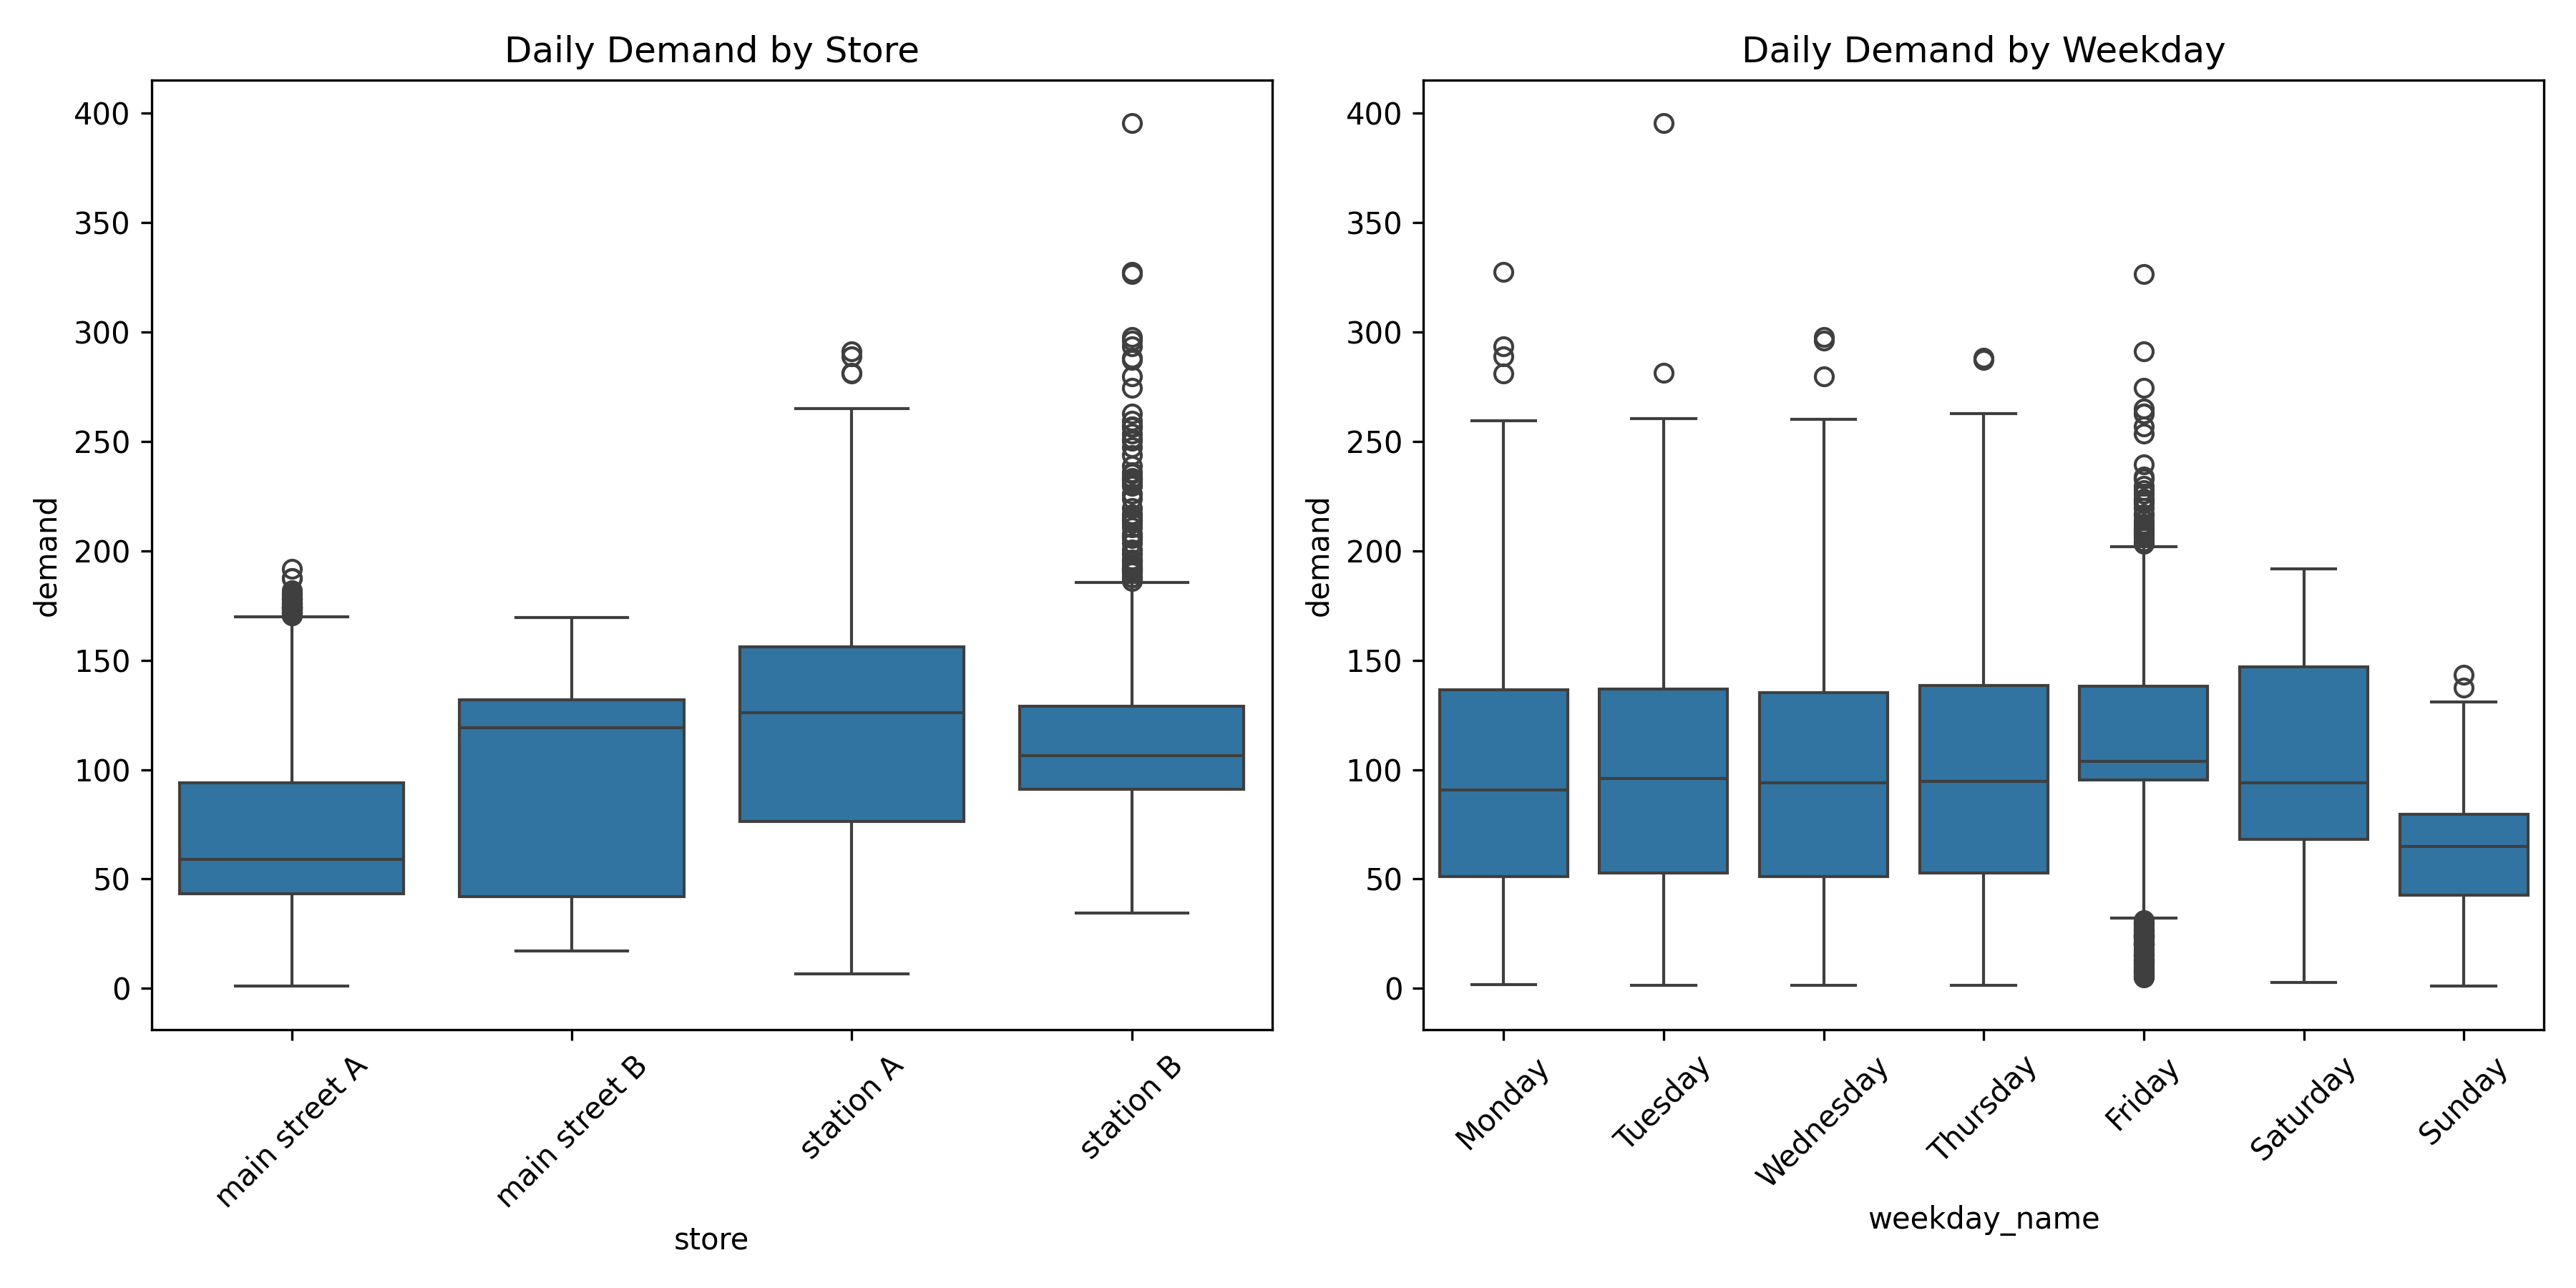
\includegraphics[width=0.95\textwidth]{figures/boxplot_store_and_weekday.png}
    \caption{Boxplot of daily demand per store and by weekday.}
    \label{fig:boxplots}
\end{figure}

\subsubsection*{b) Histograms}
Next, we plot histograms because they provide insight into the distribution of demand for each store. For example, \emph{Main Street A} exhibits a bimodal distribution, likely reflecting the variation of the demand between  weekdays and weekends, as illustrated in \cite{riley2017}, where bimodal demand patterns were observed in stores with different purchase drivers, such as weekly routine shopping versus event or project-based peaks.

Additionally, \emph{Main Street B} shows a milder bimodal pattern, which could possibly be due to the varying demand for workdays and non-workdays. This can also be observed in Riley et al. (2017), where it is discussed how stores serving multiple customer types, such as office workers versus regular passersby, often face split demand distributions.

Furthermore, \emph{Station A} displays a multi-modal and widely spread distribution, indicating inconsistent demand peaks. \cite{kharodawala2022} highlight that such demand arises in multi-modal supply chains, where the flow is influenced by unpredictable or divided demand sources, like transport hubs or event-based crowd peaks.

Finally, \emph{Station B} has a right-skewed distribution, where most daily demand values group together around a central range, but where a number of days extremely high demand spikes occur. This pattern is typical in locations exposed to irregular spikes in activity, such as transit hubs, where factors like public holidays, tourism, or transport disturbances can lead to sudden and unexpected increases. \cite{rojas2021} describe how demand skewness causes asymmetry in inventory planning, often requiring a more conservative safety stock level to guard against possible under-stocking on peak days.


\begin{figure}[H]
    \centering
    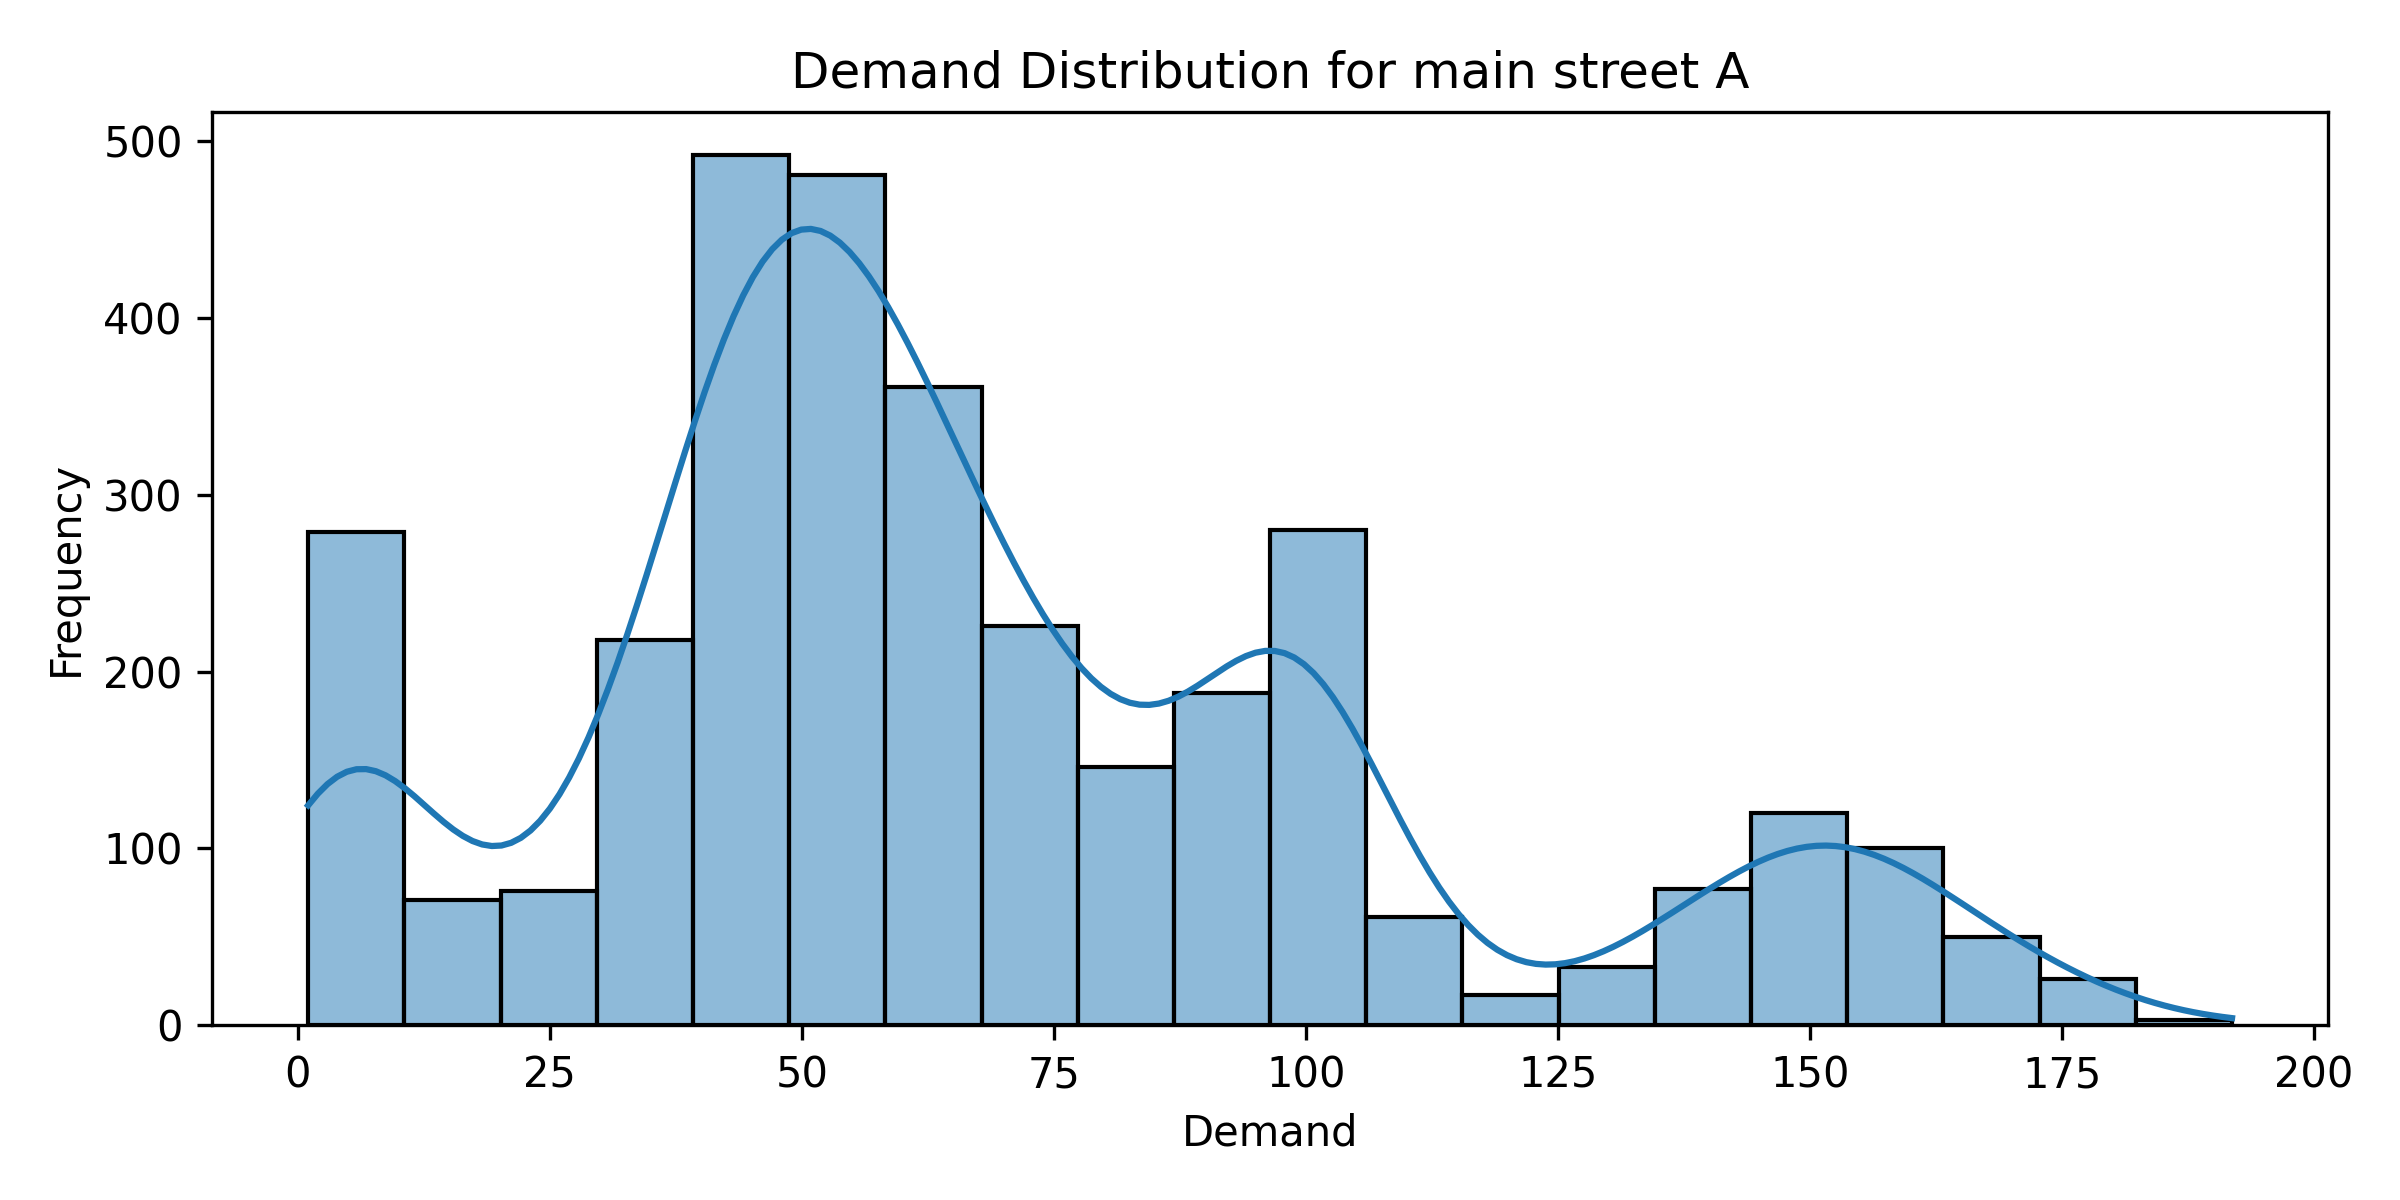
\includegraphics[width=0.49\textwidth]{figures/histogram_main_street_A.png}
    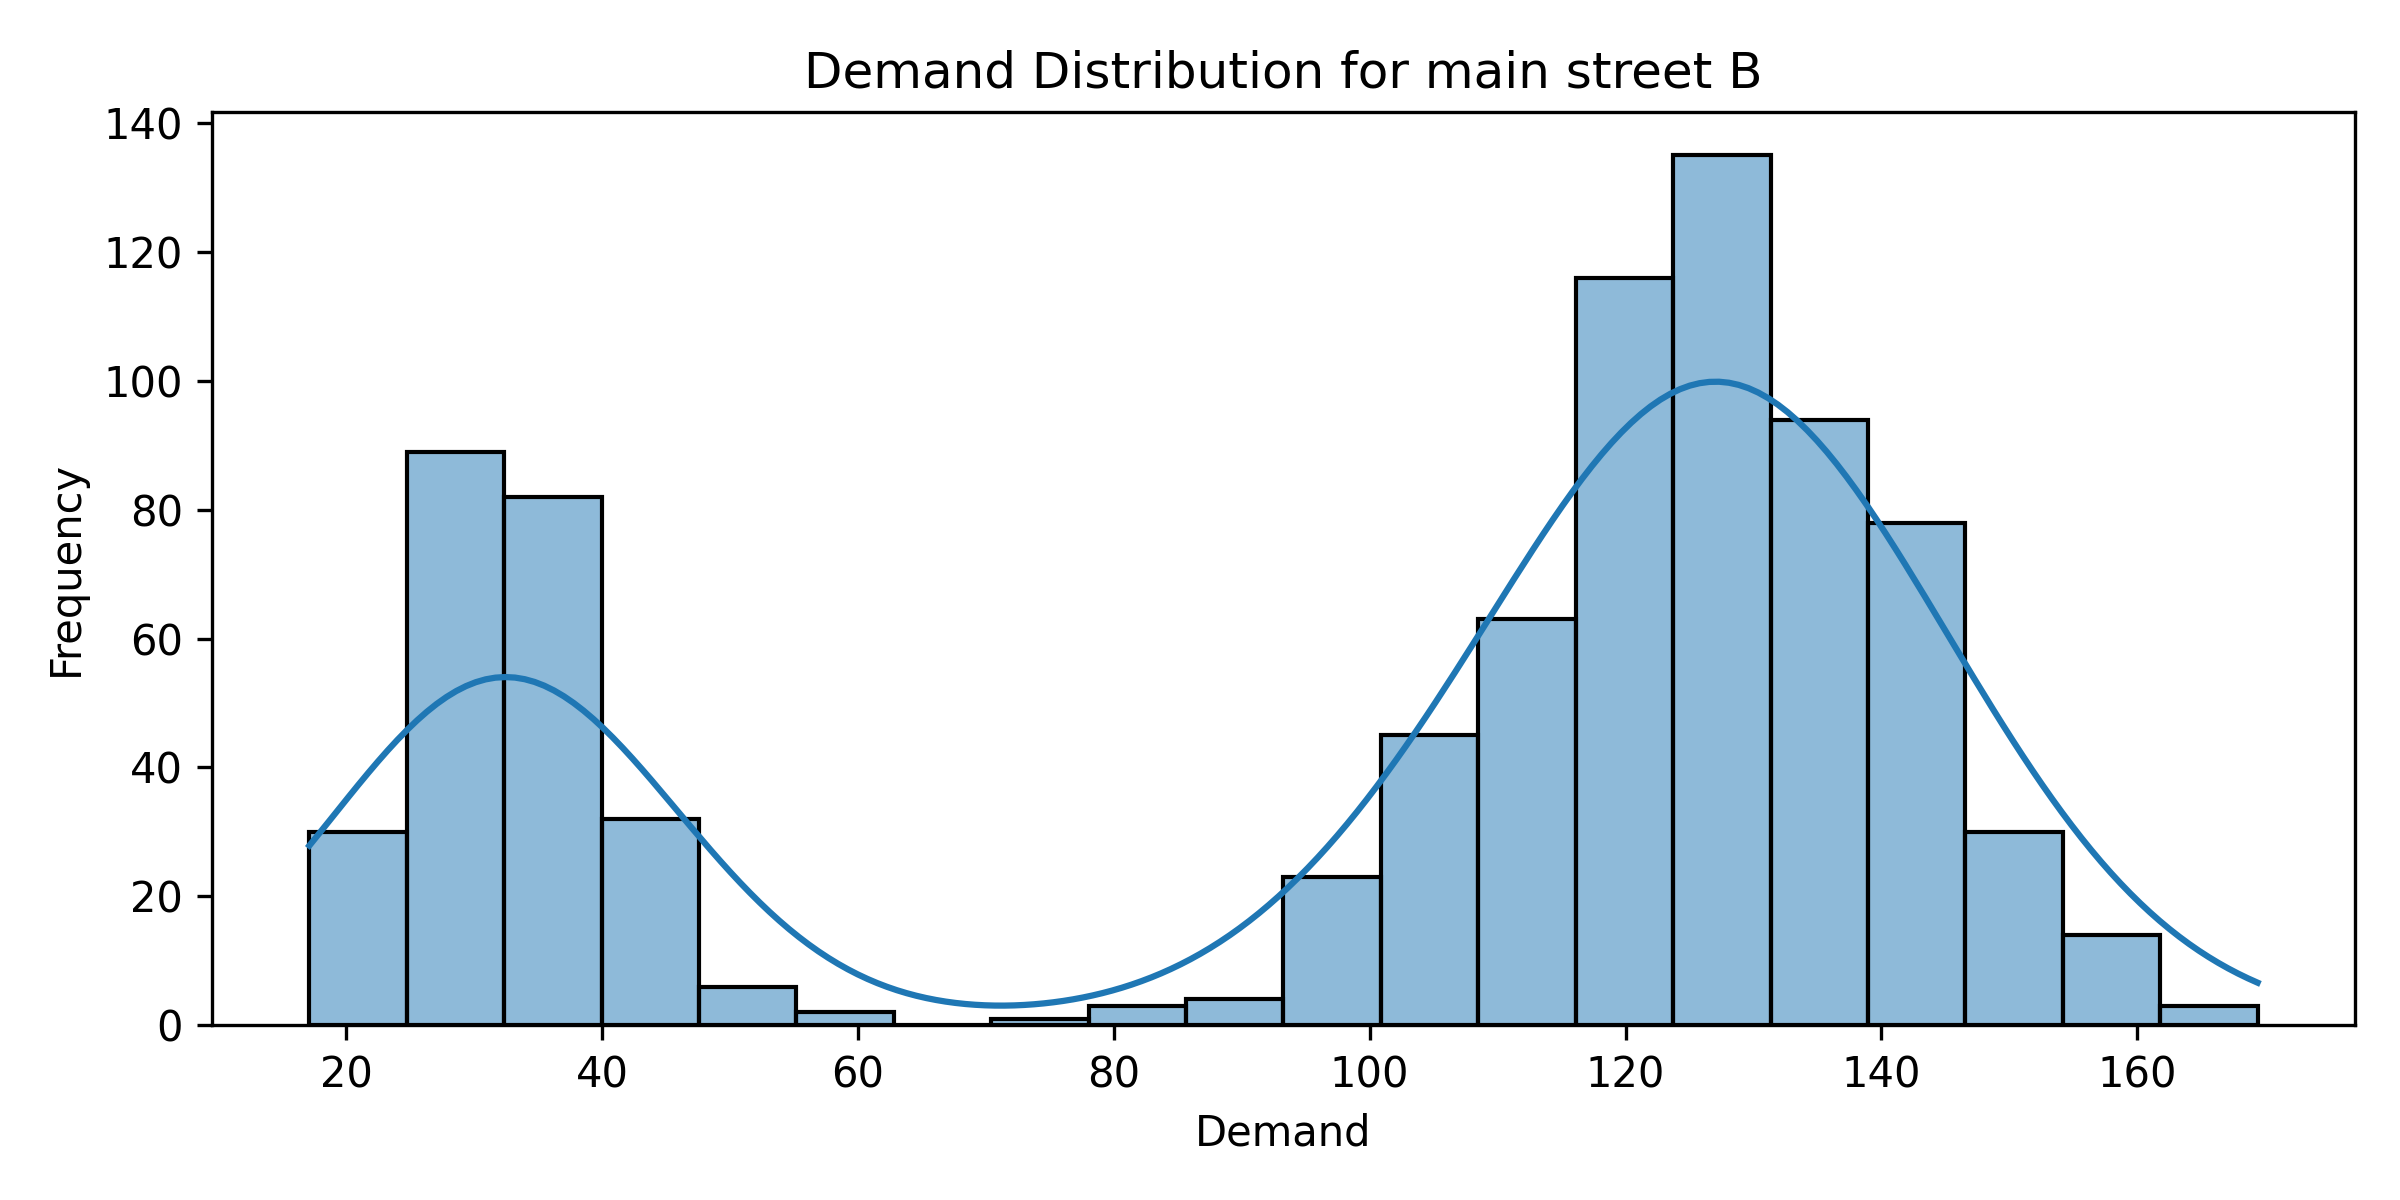
\includegraphics[width=0.49\textwidth]{figures/histogram_main_street_B.png}
    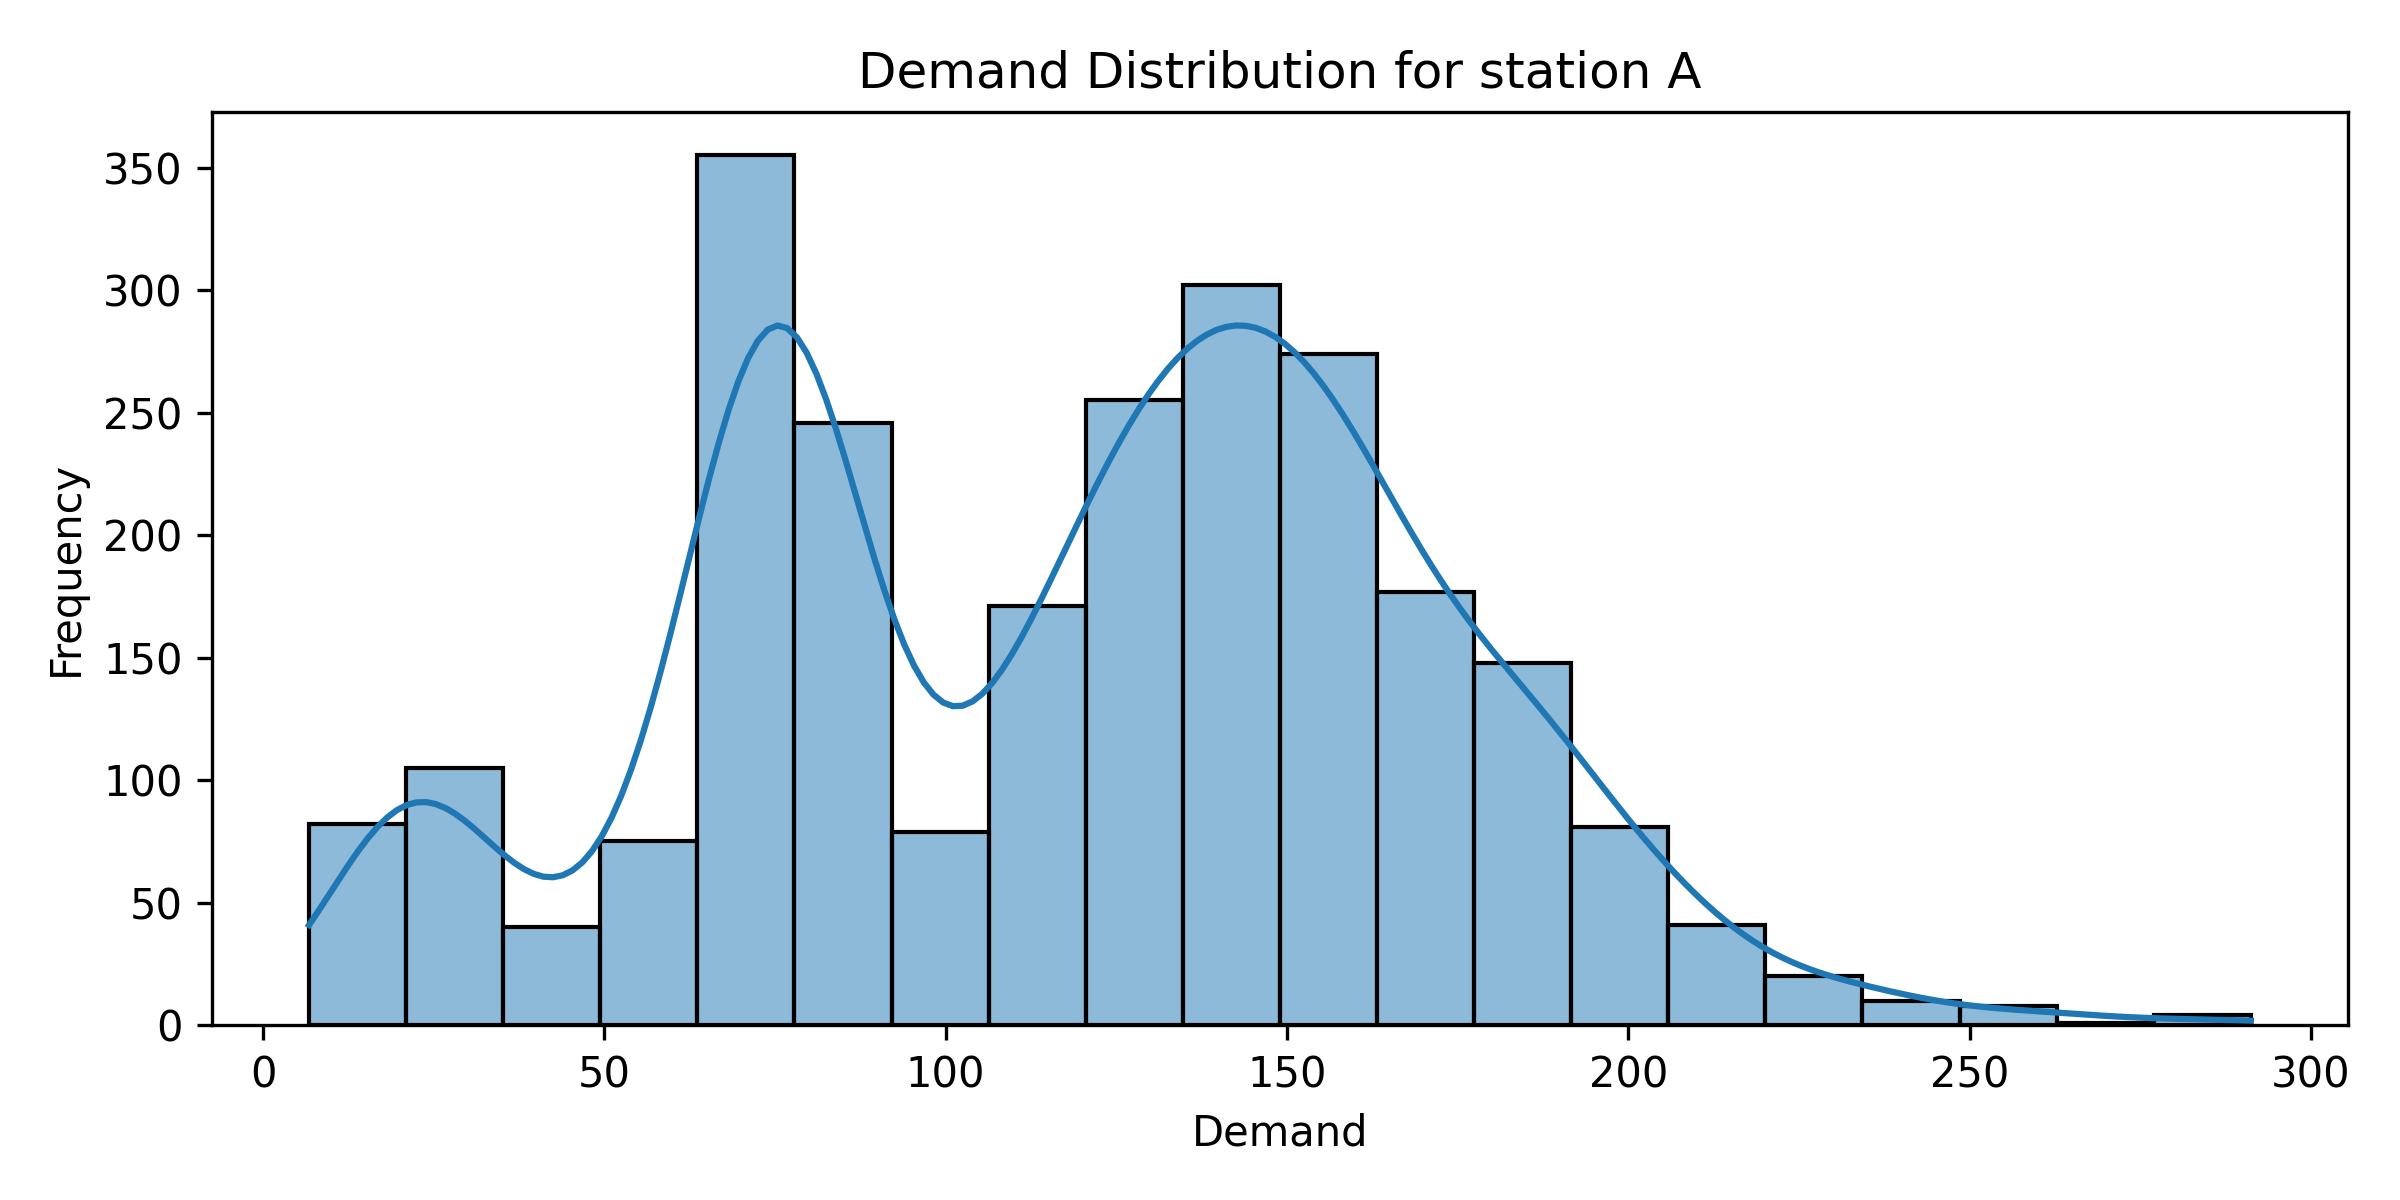
\includegraphics[width=0.49\textwidth]{figures/histogram_station_A.png}
    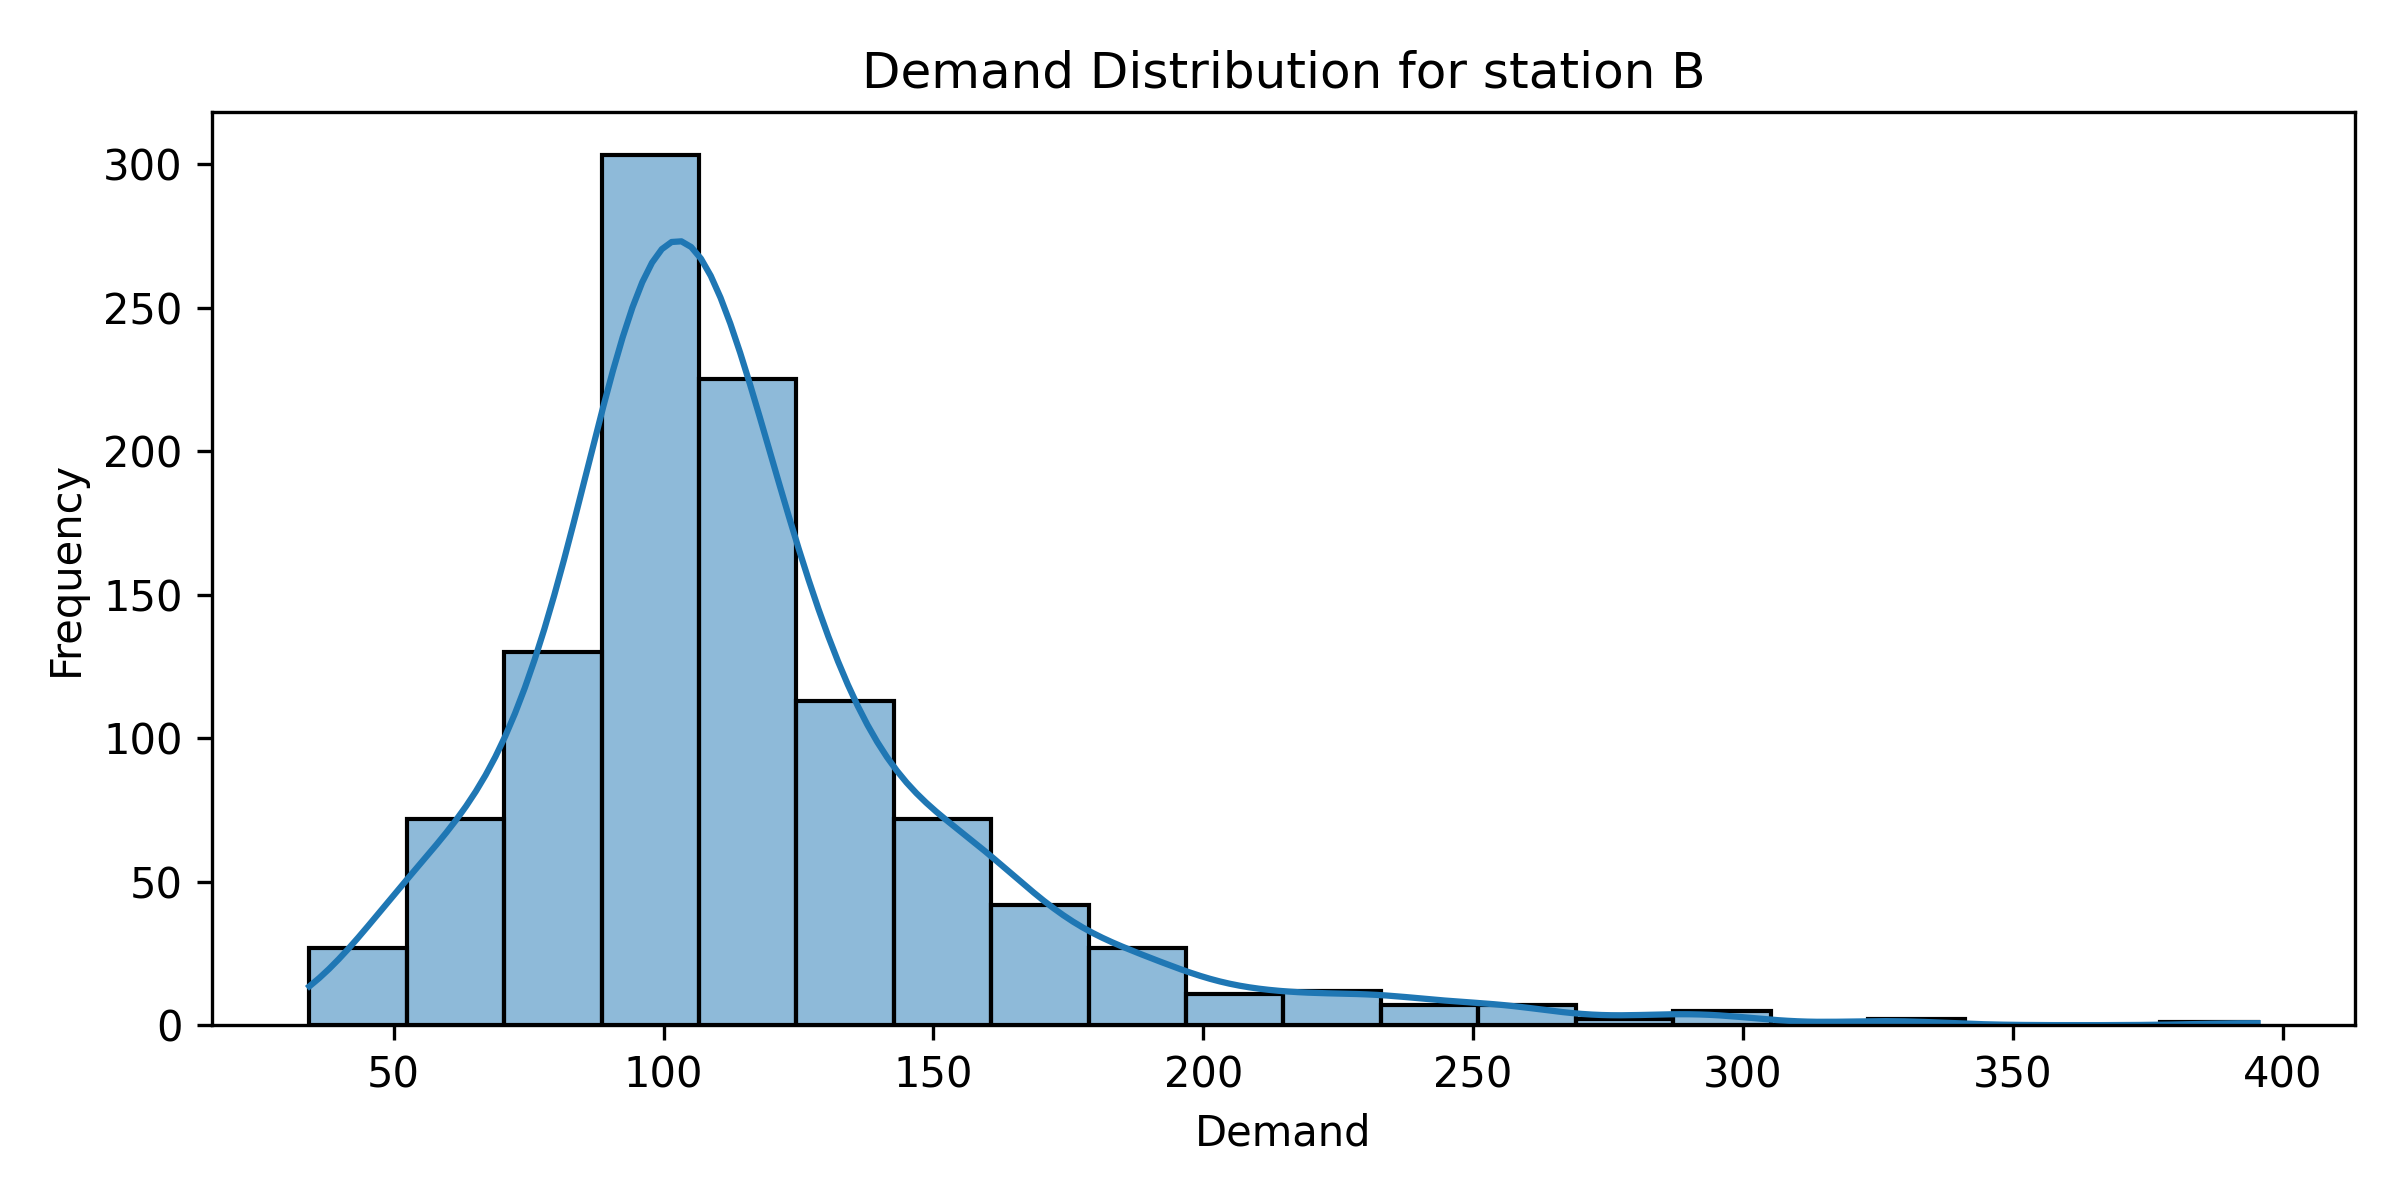
\includegraphics[width=0.49\textwidth]{figures/histogram_station_B.png}
    \caption{Histograms of demand per store.}
    \label{fig:histograms}
\end{figure}

\subsubsection*{c) Time Series Plots}
Below, the time-series plots of the stores are shown, as well as an overlay of the plots in one graph. The time series plots reveal different chronological patterns across stores that reflect on both structural and behavioral incentives of demand. 

%\emph{Main Street A} exhibits a clear COVID-related dip, while newly opened stores show more stable patterns. A weekly cycle with weekend peaks is evident across all stores. 

First, \emph{Main Street A} shows a consistent long-term trend with an obvious dip during the COVID period, followed by a gradual recovery. This pattern shows how disruptive events such as pandemics significantly reduce standard consumer activity, especially in central shopping areas (Rojas et al., 2021).

Second, \emph{Main Street B}, in contrast, shows a regular weekly cycle with little long-term movement, suggesting a stable regular weekday use likely driven by office worker habits. This is consistent with the paper of Riley et al. (2017), since it describes such repeatable demand cycles in shops in business areas, where predictable routines dominate variation.

Third, \emph{Station A} shows long-term high demand with easy observable weekly peaks and periodic peaks, which is consistent with a location highly influenced by transport flow and event-based activity. Kharodawala et al. (2021) note that retail near public transport often experiences multi-modal and unstable demand. This is a pattern that is visible in the station variability and the drop during COVID imitating \emph{Main Street A}.

Finally, \emph{Station B} presents a clearly unstable time series with frequent spikes, but its 7-day average shows a relatively stable trend. This supports the histogram's indication of the right-skewed demand. According to Rojas et al. (2021), this is typical in systems where external shocks, travel behavior, or seasonal effects occasionally raise demand.

As a result, the combined time series plot highlights clear contrasts between stores: the station stores show higher variability and demand peaks, while the main street stores show a smoother and a more regular pattern. The COVID drop is visible in all locations, but its impact was most noticeable in \emph{Main Street A}, highlighting the sensitivity of retail stores in the city to external shocks.




\begin{figure}[H]
    \centering
    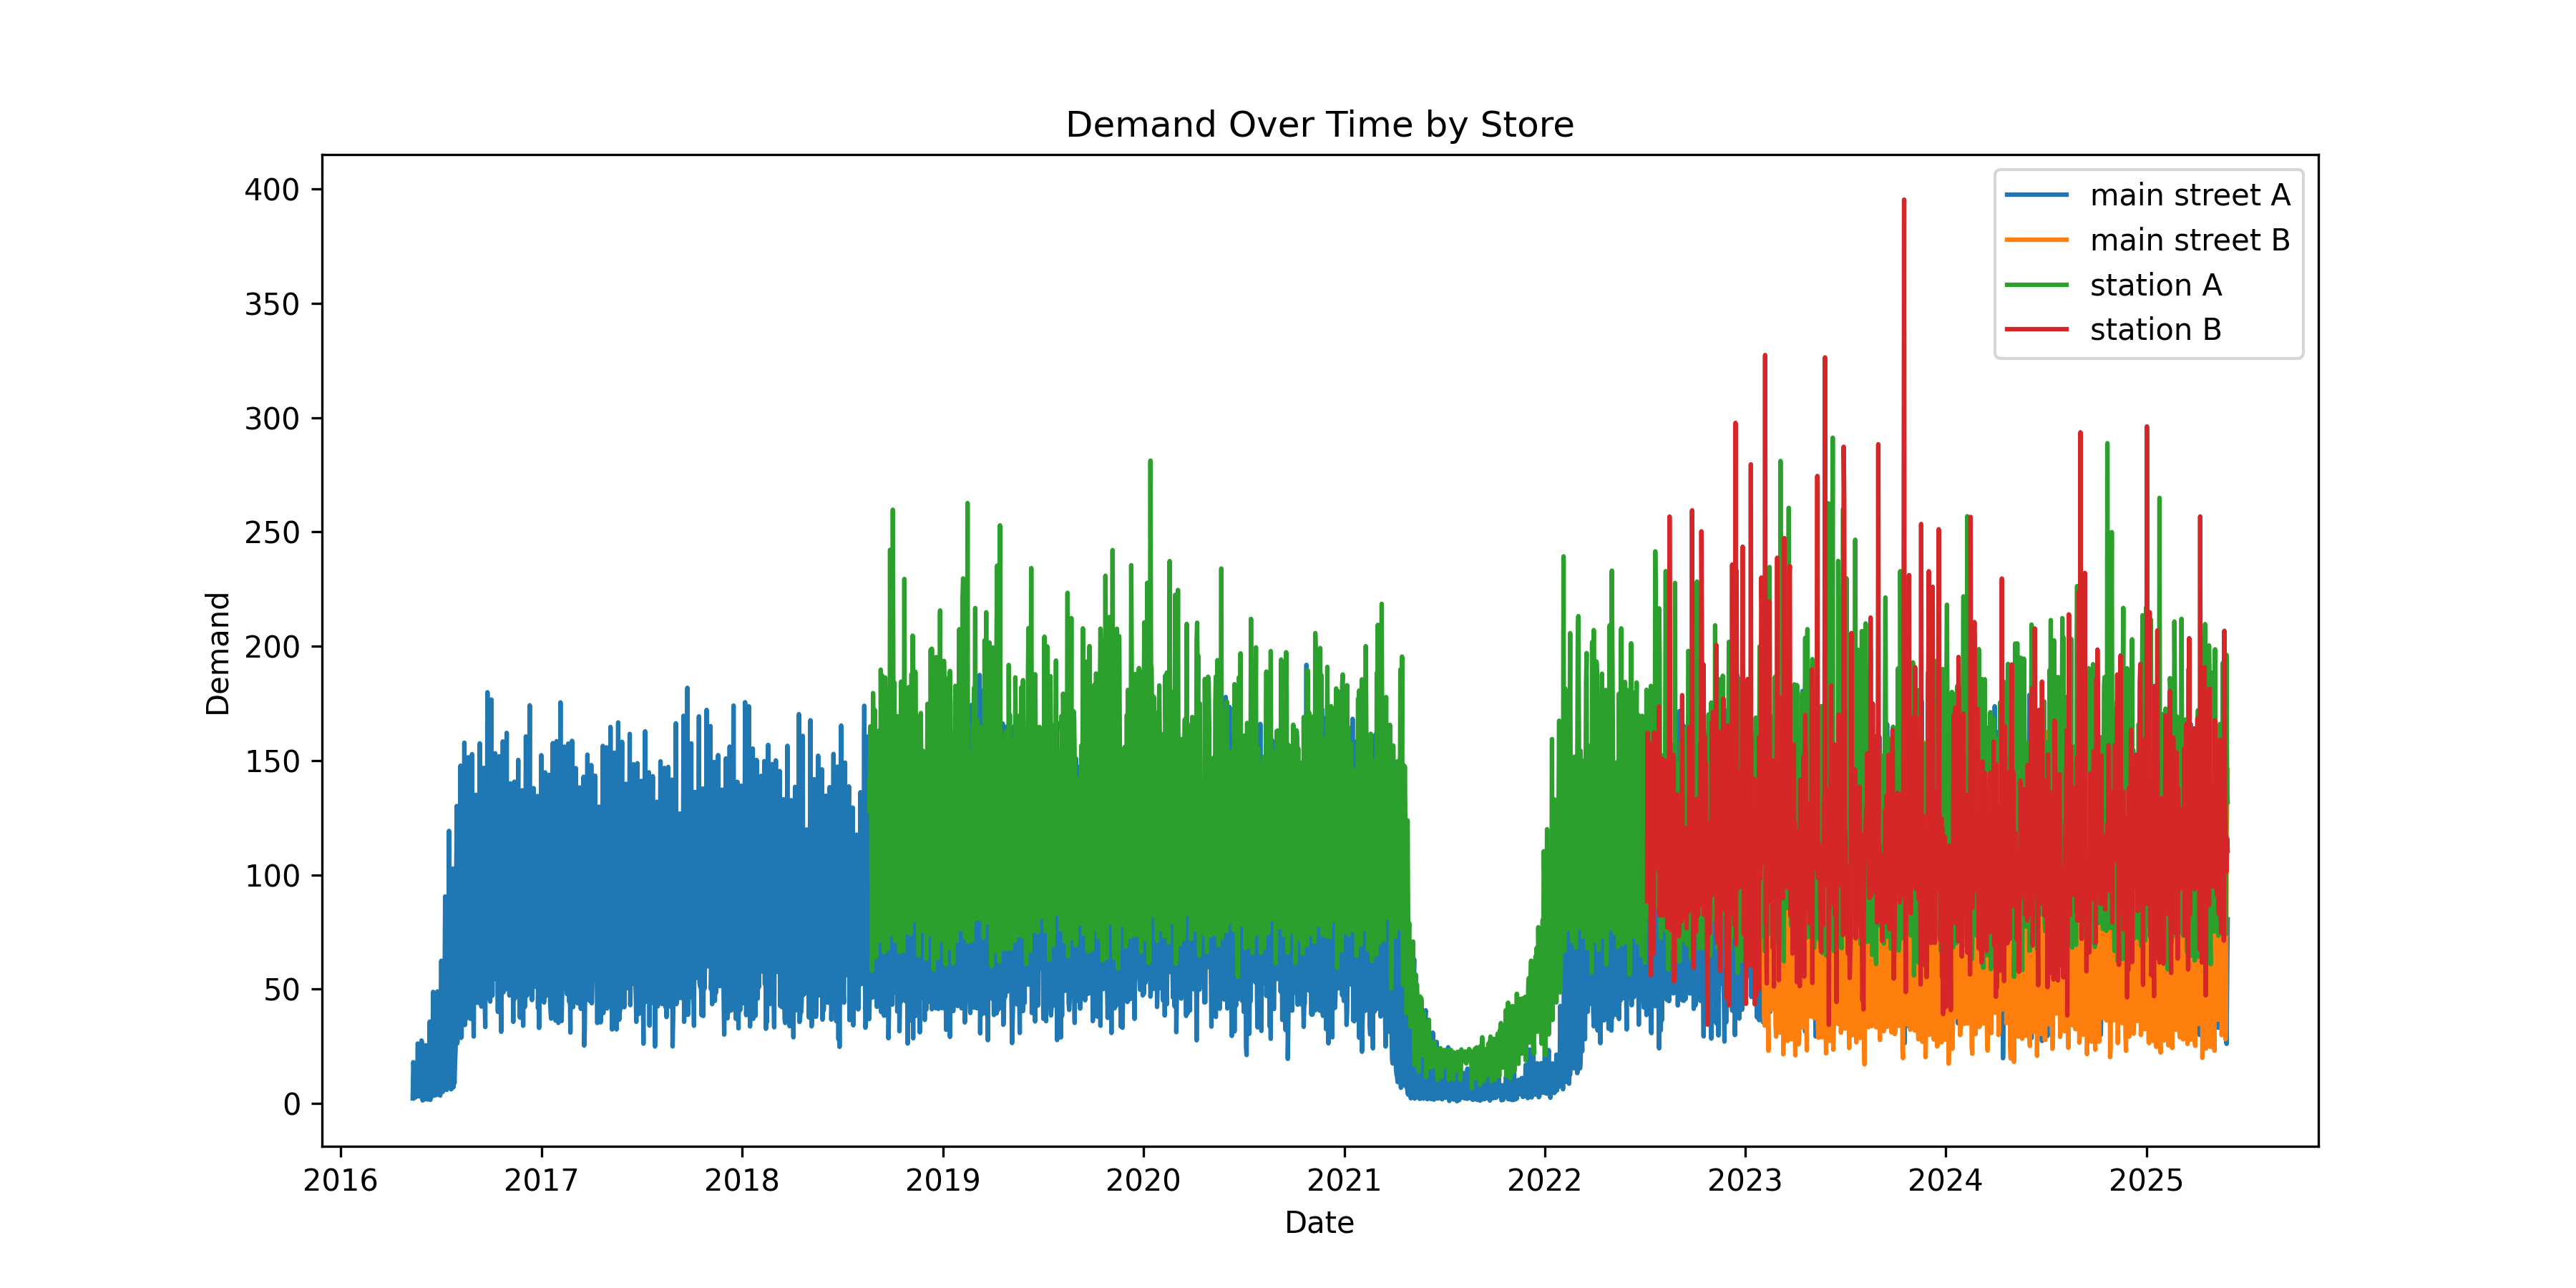
\includegraphics[width=0.95\textwidth]{figures/time_series_all_stores.png}
    \caption{Daily demand over time for all stores.}
    \label{fig:all_timeseries}
\end{figure}

\begin{figure}[H]
    \centering
    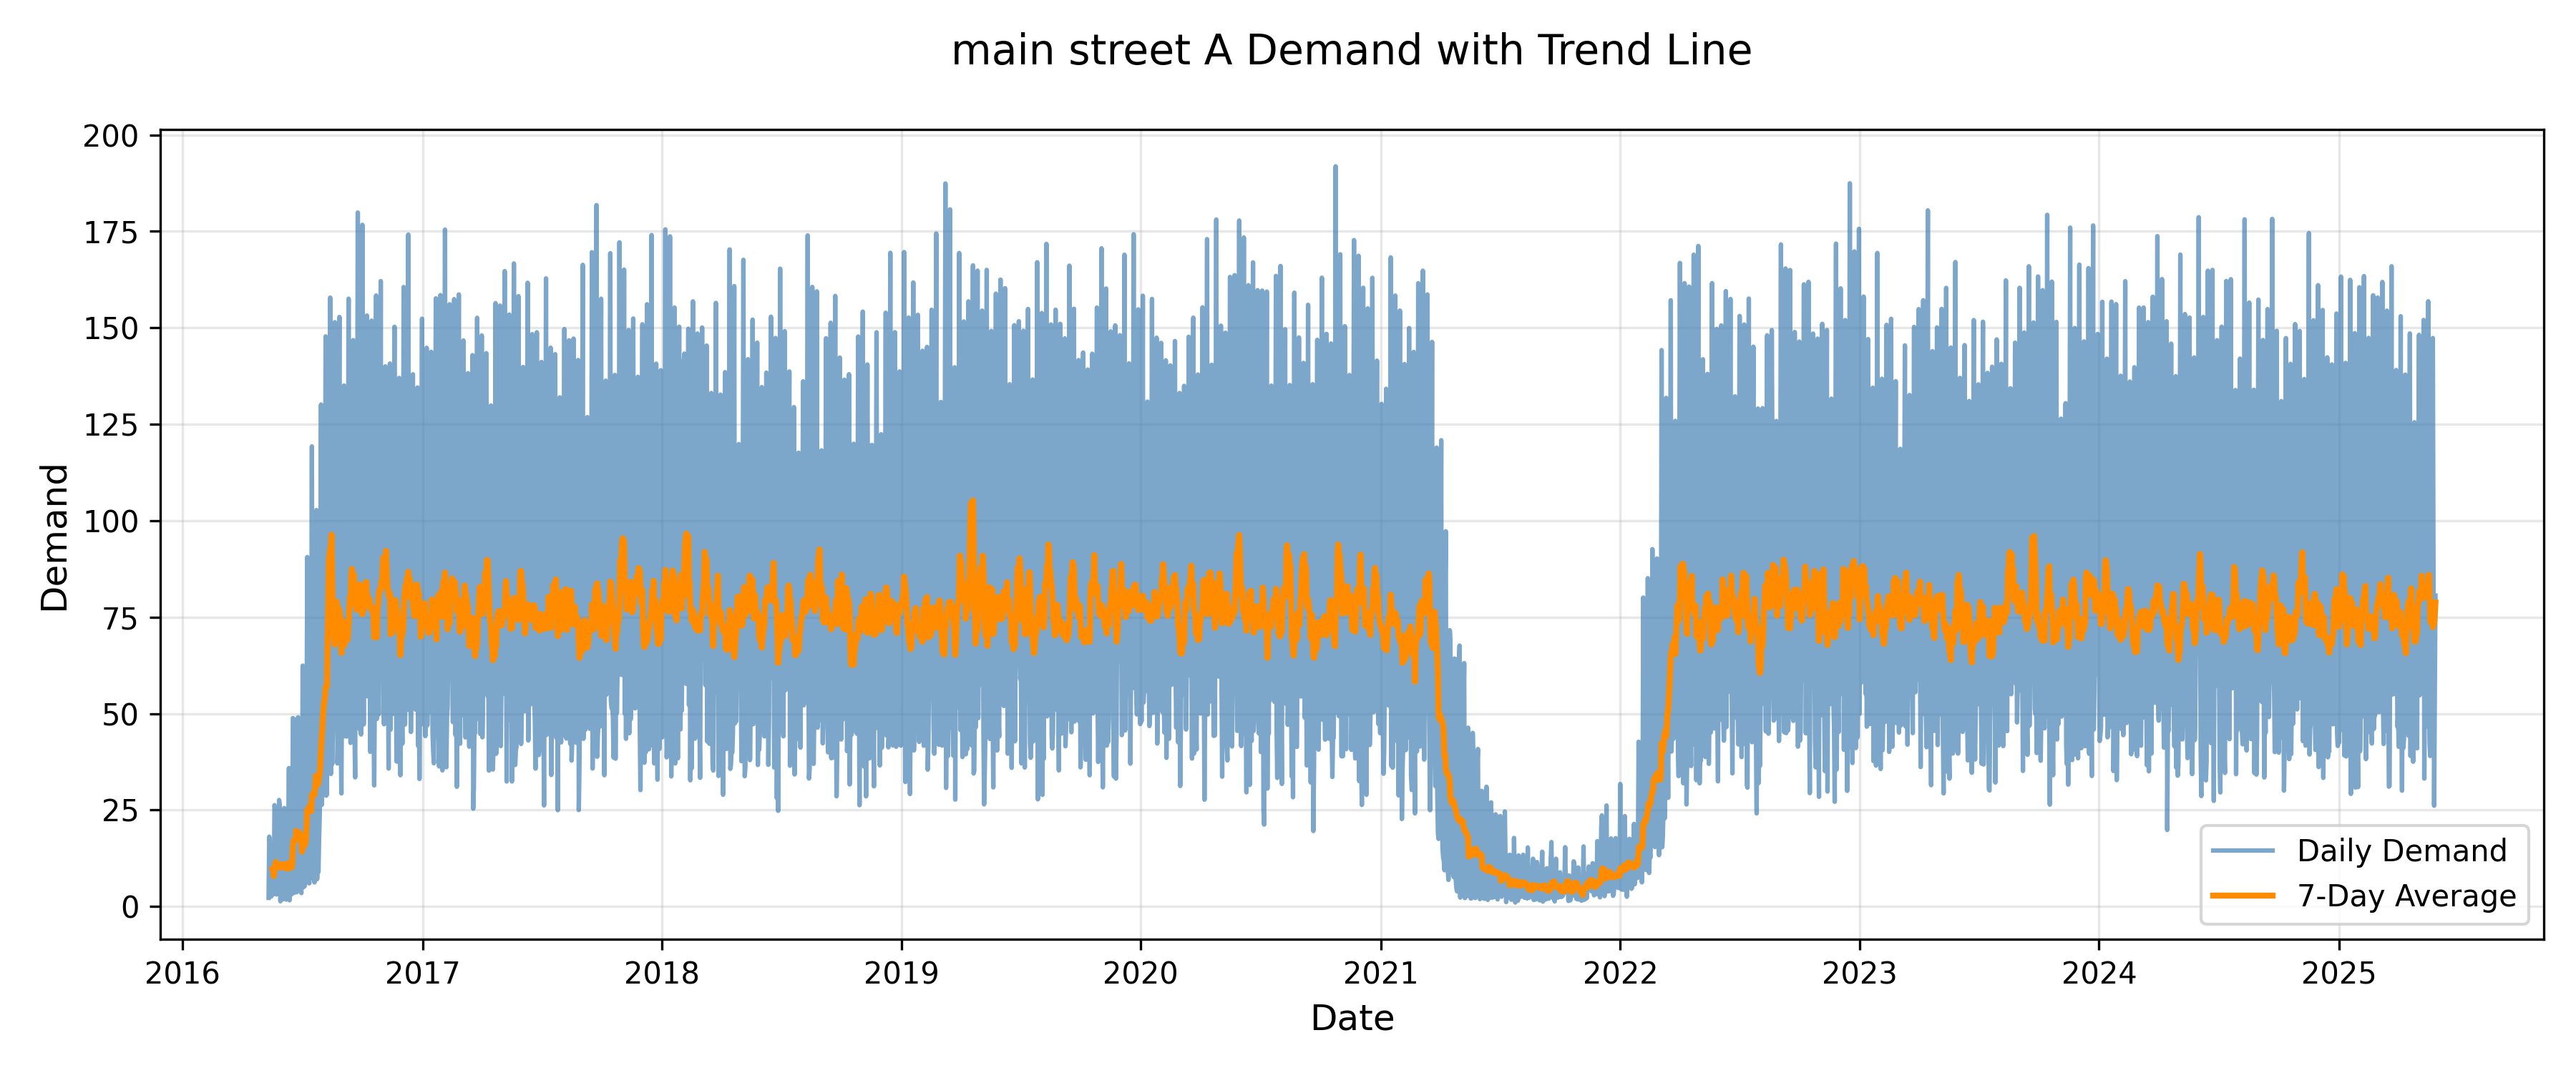
\includegraphics[width=0.48\textwidth]{figures/store_trend_main_street_A.png}
    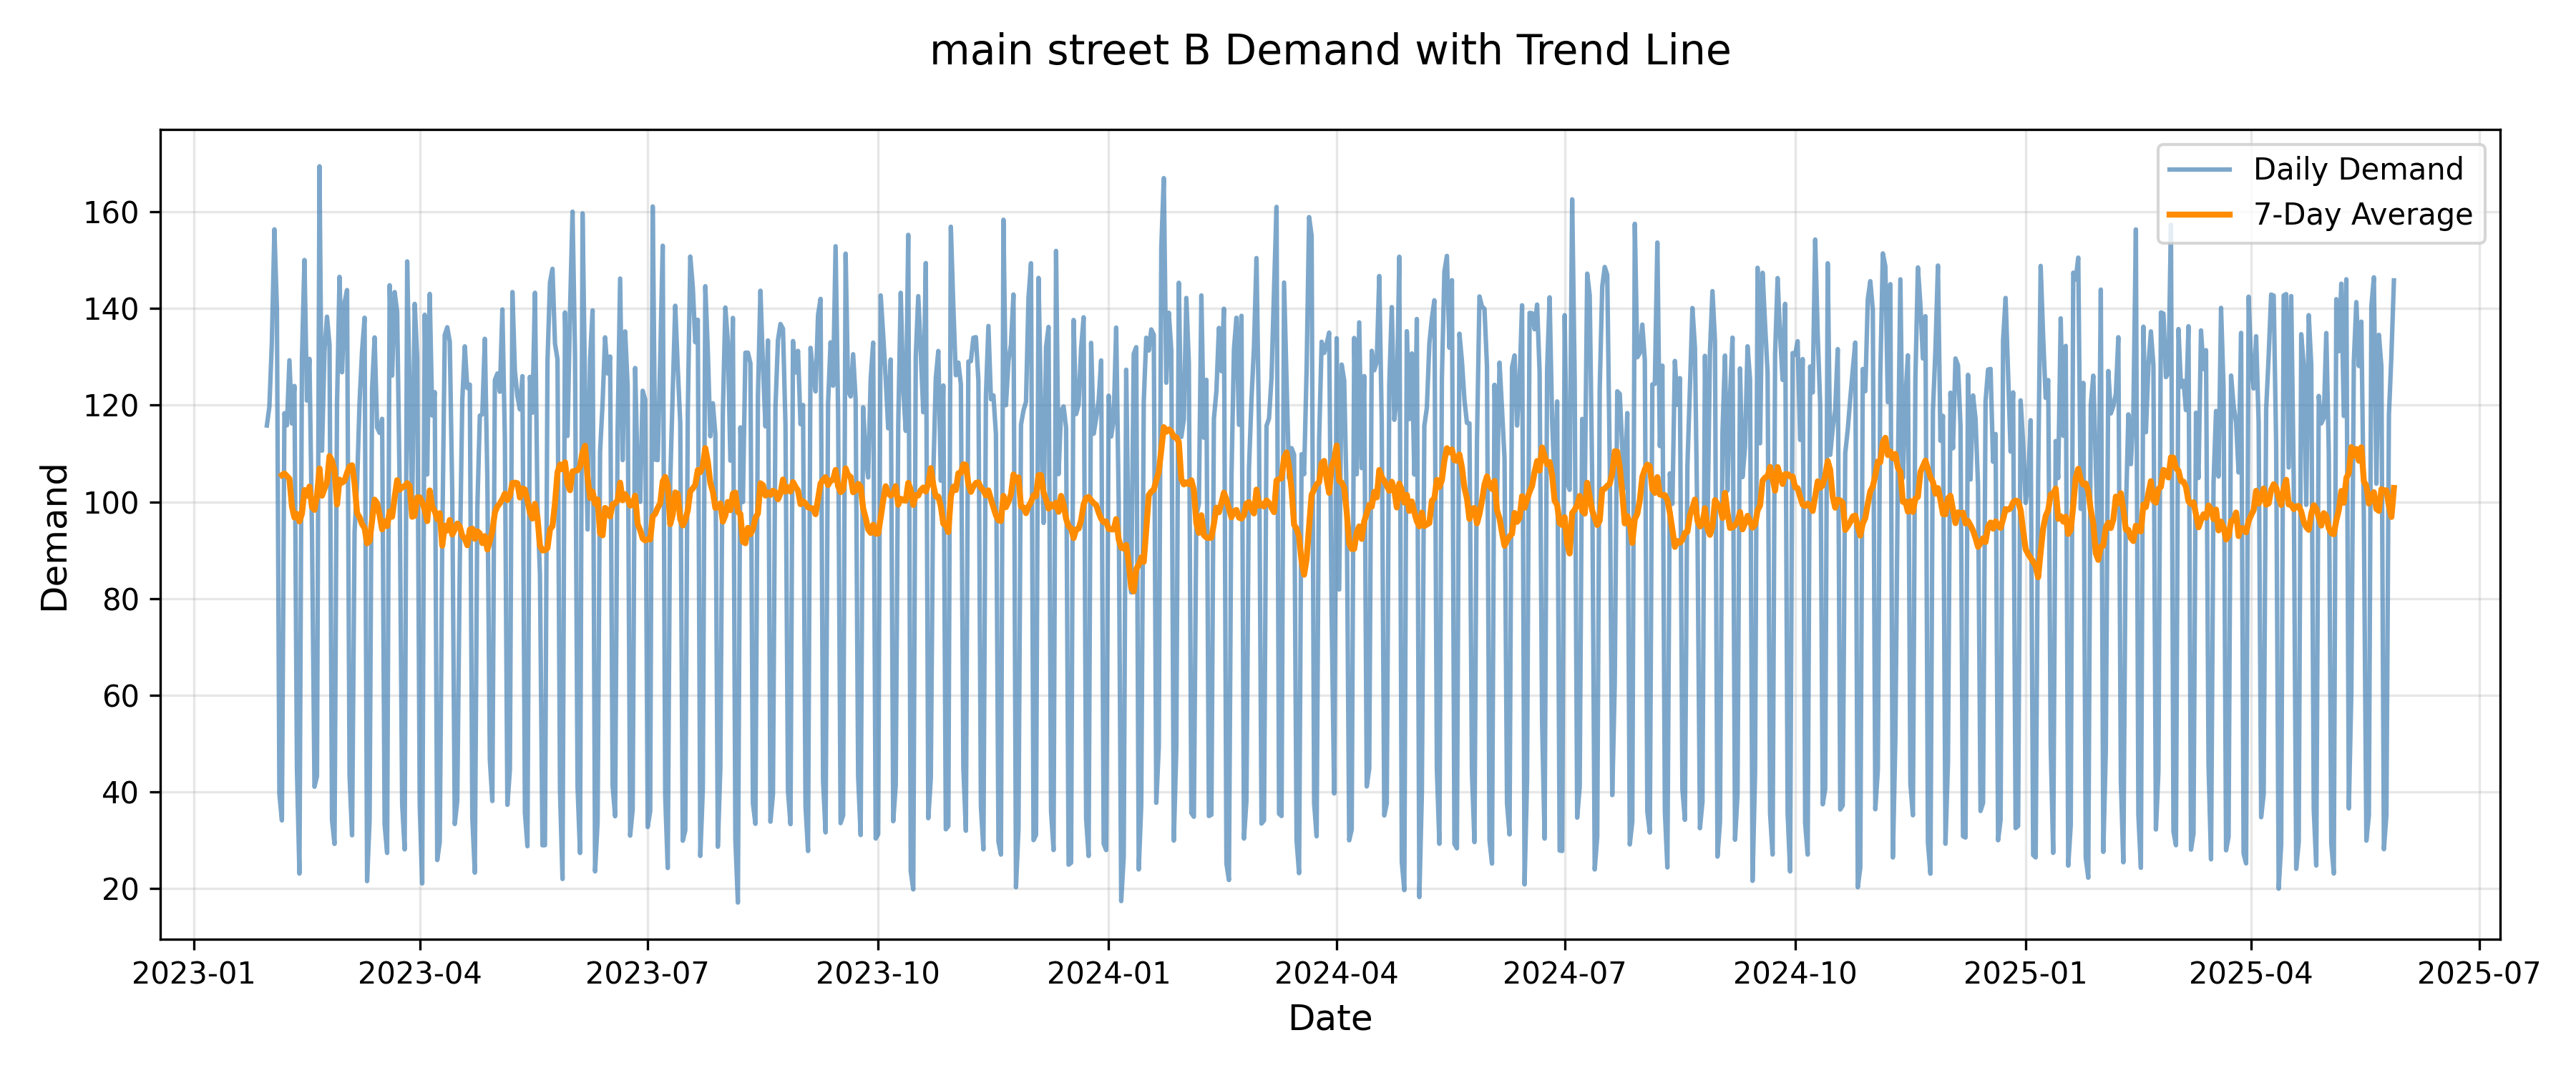
\includegraphics[width=0.48\textwidth]{figures/store_trend_main_street_B.png}
    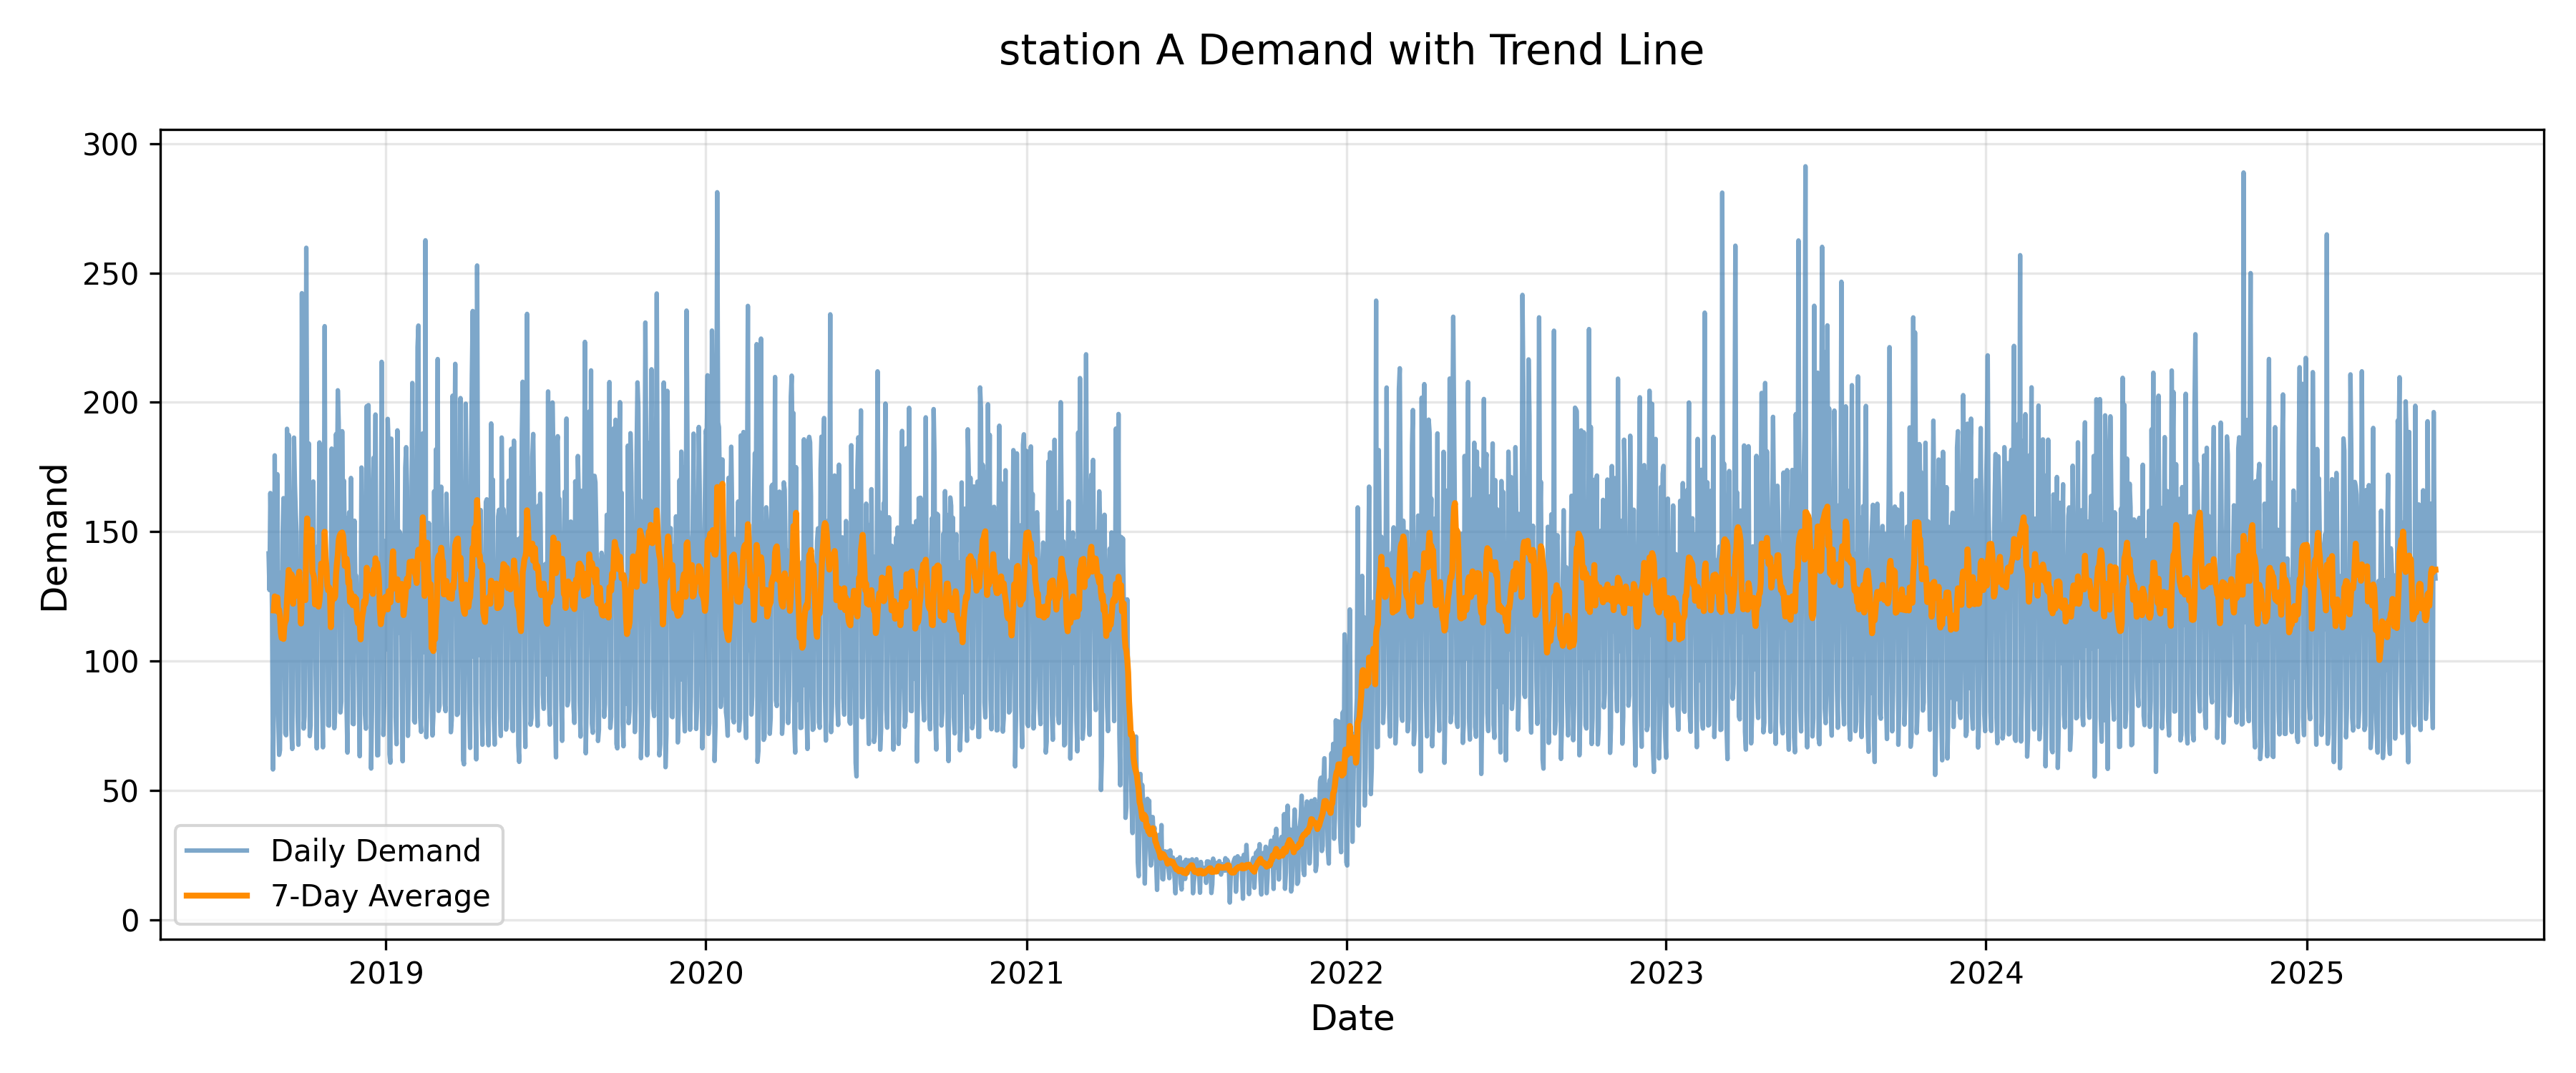
\includegraphics[width=0.48\textwidth]{figures/store_trend_station_A.png}
    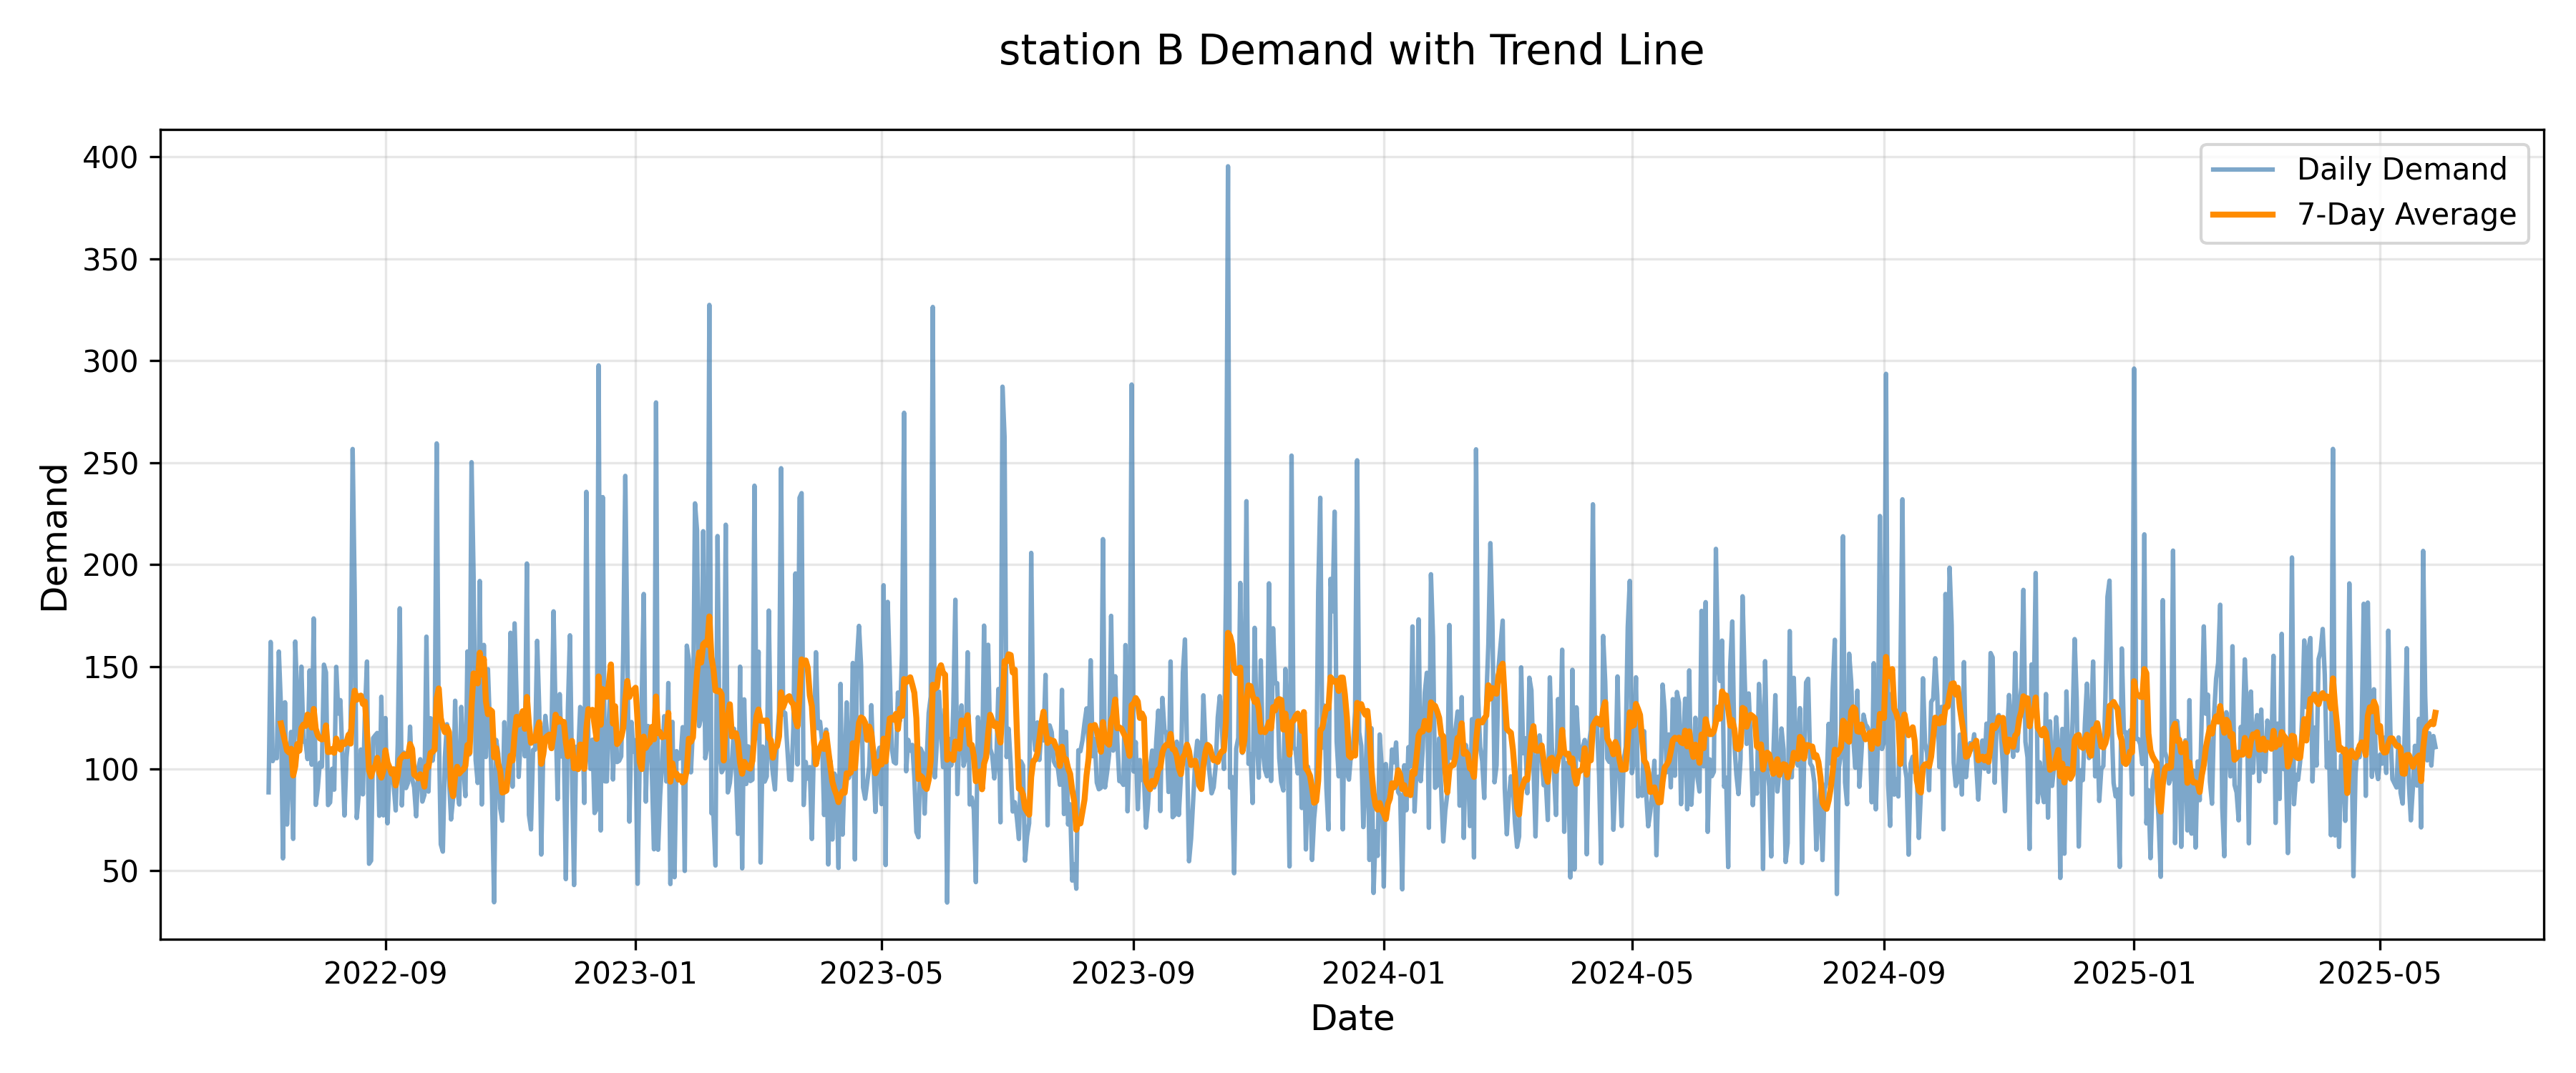
\includegraphics[width=0.48\textwidth]{figures/store_trend_station_B.png}
    \caption{Daily demand and 7-day moving average per store.}
    \label{fig:trend_lines}
\end{figure}


\section*{Task 6: Parametric Framework}
\subsubsection*{a) Choice of Stores}
\medskip
For this analysis, we have selected two stores. The first store will be \emph{Main Street A}, as this store is located in a high-traffic shopping area with an established demand affected by seasonal variation and was established before COVID and has survived COVID. 

The second store that has been selected is \emph{Station B}. Since this is a newer location near a transport hub, it shows more irregular and yet high demand levels and has a right-skewed distribution.

Because \emph{Main Street B} is relatively stable, has a lower average demand and has fewer distinguishing characteristics, it would not add any analytical contrast to the two selected stores.

In addition, \emph{Station A} is also located in a high traffic zone. The store presents a more complex multi-modal distribution and has a higher day-to-day variability, which may make it less relevant for reliable parametric modeling. 

By selecting \emph{Main Street A} and \emph{Station B}, we capture the contrast between a steady, well-understood location and a newer, high-variance location, which allows us to demonstrate how different distributional assumptions apply across different demand contexts.

\subsubsection*{b) Specification of Demand Distributions}
\medskip

To specify the demand distributions, we look back at the results from task 5, since that is where we analyzed the shape of the demand using histograms, box plots, and time series visualizations from all stores. 

For \emph{Main Street A}, the histogram looked like a bimodal distribution, probably driven by the differing behavior of the customers between weekdays and weekends. However, when the data are filtered by individual weekdays, the demand appears to be approximately normally distributed. Hence, the use of a \textbf{normal distribution} as a reasonable parametric approximation is logic for short-term forecasting, especially when adjusting for the day of the week. 
This choice is further supported by \cite{ramaekers2008}, who write in their paper that when the mean demand is relatively high compared to its variance, as in the case for Main Street A, the normal distribution can serve as a suitable approximation in inventory models. For example, on Fridays, the demand at the store \emph{Main Street A} shows a high concentration around the center and relatively low skewness, which aligns well with the conditions under which a normal model performs consistently.

For \emph{Station B}, Task 5 shows a right-skewed distribution with a high concentration of average demand days and some rare sharp peaks. This pattern can be seen in the histogram, as well as in the box plot and time series plot. Based on this, we choose a \textbf{log-normal} distribution to capture the positive skewness and the scaling effect of high-demand conditions. The log-normal model is particularly suitable for nonnegative, right-skewed shopping demand (\cite{rojas2021}).


\subsubsection*{c \& d) Point Estimates and Intervals for the Theoretically Optimal Quantities}
\medskip

In this section, we estimate the optimal order quantities $Q^*$ for the short term, by using the Normal and Log-Normal parametric approach. These estimates are based on the critical fractile formula, which has been derived in section 2. These incorporate adjusted cost values $\tilde{c}$ that incorporate the clearance price and the shipping costs.

The following table summarizes the point estimates and the 95\% confidence intervals for the \emph{Main Street A} store for the different weekdays.

\begin{figure}[H]
    \centering
    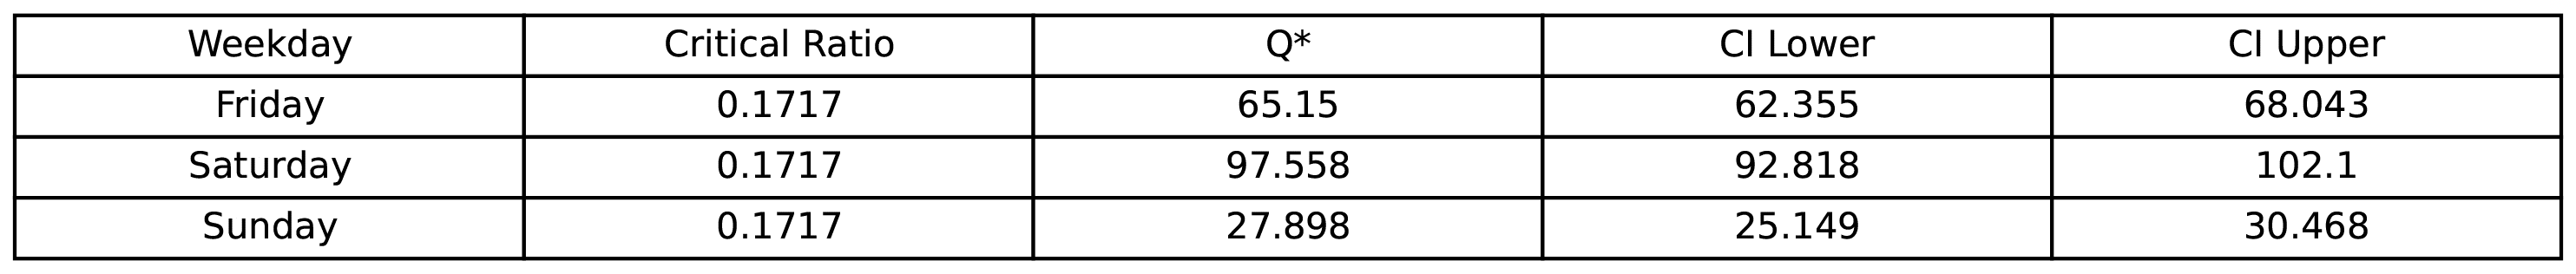
\includegraphics[width=1\textwidth]
    {figures/Figure_Normal_MainStreetA.png}
    \caption{Table of point estimates and confidence intervals for Main Street A with normal distribution}
    \label{fig:Table for Main Street A}
\end{figure}

For Main Street A, the demand is more predictable and increases on weekends, with its peak on Saturday at 97.56 units, while remaining mild on Friday, with 65.15 units, and quite lower on Sunday, with 27.90 units. The tighter confidence intervals reflect consistent and well-distributed foot traffic. This pattern is typical for stores located in shopping districts, where the demand tends to be more stable and evenly distributed throughout the day and week due to flexible and recreational shopping behavior (\cite{berry2016}).

Next, in the following table, the point estimates and the 95\% confidence intervals for the \emph{Station B} store are shown for different weekdays.

\begin{figure}[H]
    \centering
    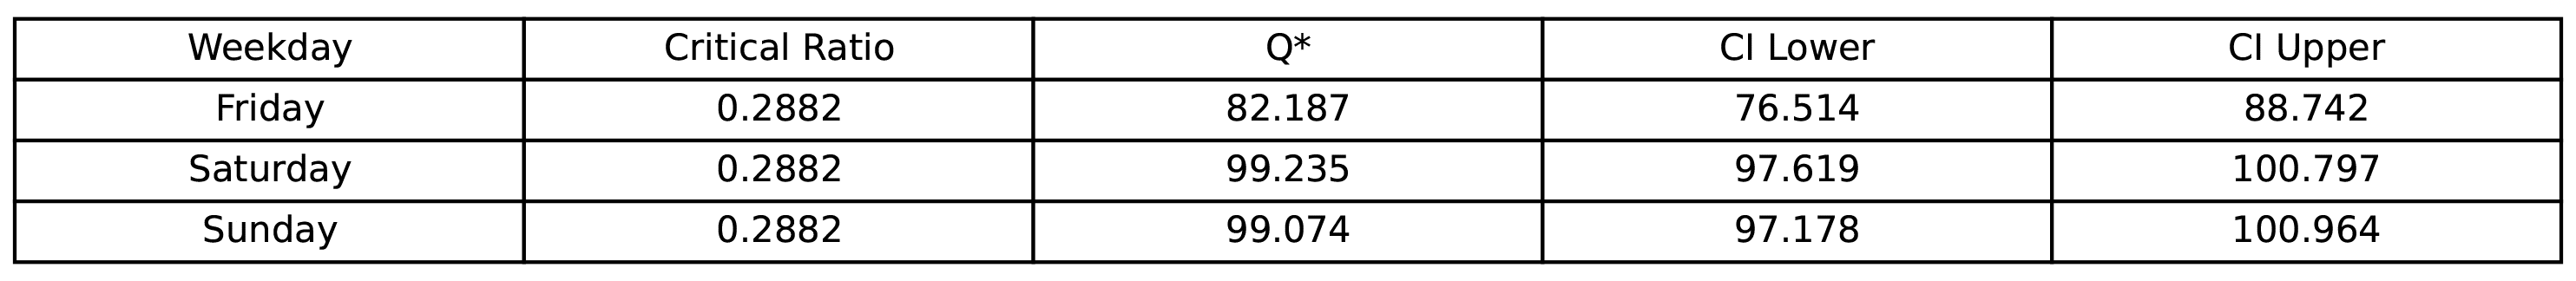
\includegraphics[width=1\textwidth]
    {figures/Figure_LogNormal_StationB.png}
    \caption{Table of point estimates and confidence intervals for Station B with lognormal distribution}
    \label{fig:Table for Station B}
\end{figure}

In contrast, Station B shows a higher and more volatile demand, with estimates almost being equal on the weekends and on Friday a little lower with 82.19 units. The narrow confidence intervals on weekends indicate a concentrated but predictable peak behavior. These patterns are in line with the findings of Berry et al. (2016), who note that shops near transport hubs experience highly time-specific demand peaks driven by transit flows, leading to a right-skewed and more variable demand distribution.
In general, the variation in the choice of the distributions and the resulting estimates is based on the spatial context of each store. This confirms that inventory strategies must be different for each location and driven by data.

\section*{Task 7: Price Sensitivity Analysis}
The stated goal of this task involved conducting an analysis to determine the optimal price increase to maintain current profit levels, under the expectation of a 25\% increase in operational costs. This analysis was carried out with an 8-function Python script. A detailed summary of each function, including its name, input parameters, and purpose, is presented in Table~\ref{tab:functions}.

This analysis was conducted under the assumption that, for each price increase considered, the bakery would also adjust its order quantity optimally, thereby minimizing losses due to under- or overstocking. Furthermore, profit deviations (whether above or below current levels) were treated symmetrically, as the primary goal was to maintain current profit levels rather than to maximize profit under the new cost burden.

The order of analysis started by first scaling the operational costs per store by a factor of 1.25, resembling the expected 25\% increase. After this, the expected percentage decrease in demand (\( rY \)) corresponding to a given percentage increase in price (\( rP \)) was calculated, using a formula (Fig.~\ref{fig:demand_drop}) provided by the bakery’s internal research team. Historical demand data for each store was then adjusted downward using a scaling factor of \( 1 - \frac{rY}{100} \), to simulate the impact of price sensitivity on consumer behavior. Based on the adjusted demand, the optimal order quantity (\( Q_{\text{new}} \)) was recalculated using the non-parametric function developed in the previous task. This step ensures that inventory decisions remain consistent with changes in decreased customer demand resulting from price increases, thereby providing a more realistic simulation of the relationship between pricing strategy and consumer behavior. To isolate the effect of the price increase on profitability from the confounding effect of also changing the demand, two parallel analyses were conducted: one assuming dynamic demand (where both demand and order quantity vary with \( rP \), reflecting a realistic scenario), and another with static demand (holding both demand and order quantity constant, to assess the direct financial impact of the cost and price changes in isolation).

\begin{figure}[h]
    \centering
    \caption{Demand Drop Formula (\( rY \))}
    \label{fig:demand_drop}
    \[
    rY = \left[ \left[ 1 + \exp\left(6 - \frac{rP}{10}\right) \right]^{-1} - 0.0025 \right] \times 100
    \]
\end{figure}

The next stage of the analysis involved comparing current profit levels (before the 25\% increase in operational costs and any price adjustments) with the expected profit levels resulting from different price increases (\( rP \)). Once again, two separate approaches were considered. The first analysis assumed that the bakery would continue its policy of uniform pricing across all store locations. In this scenario, the current profit level was calculated as the average profit across all stores, and each \( rP \) was evaluated by comparing this average to the average expected profit across all stores after the cost increase. Upon closer inspection, it became evident that while some stores remained highly profitable, others operated at a loss. These losses were effectively masked by the strong performance of the more profitable locations, leading to a misleading aggregate view.  Hence, assuming the bakery owners would like to keep each store profitable, a second approach was used. The second analysis ignored the uniform pricing assumption and evaluated each store independently. Here, the current profit for each store was individually compared to its expected profit under different \( rP \) values. This approach resulted in different optimal price increases per store and provides an alternative strategy for the bakery should it choose to abandon its same-price policy.

\renewcommand{\arraystretch}{1.4}
\begin{table}[H]
\begin{tabular}{|>{\columncolor{blue!20}}p{6cm}|p{5cm}|p{5cm}|}
    \hline
    \rowcolor{black!10}\textbf{Function name} & \textbf{Function Parameters} & \textbf{Function Purpose}  \\ \hline
    calculateDemandDrop & rP (percentage increase) & Computes the demand drop percentage from the price increase. \\ \hline
    adjustDemand & vY0 (original data set), rY (demand drop percentage) & Scales demand data by demand drop factor. \\ \hline
    nonparametricBootstrapCi & data (Demand data array), cr (Critical ratio (0–1)), alpha (Confidence level, default 0.05), B (Bootstrap iterations, default 1000) & Estimates quantile and confidence interval via bootstrap. \\ \hline
    calculateOptimalOrderQuantity & dfadjusted (Adjusted demand DataFrame), criticalratio (Critical ratio value) & Determines optimal order quantity per store using bootstrap. \\ \hline
    computeCurrentProfit & df (Demand data DataFrame), Q (Order quantity dictionary), c0 (Current cost dictionary), p0 (Current price dictionary), pL (Lowered price dictionary), cS (Shipping cost dictionary) & Calculates current profit for each store. \\ \hline
    computeNewProfit & dfadjusted (Adjusted demand DataFrame), Q (Order quantity dictionary), c1 (New cost dictionary), p1 (New price dictionary), pL (Lowered price dictionary), cS (Shipping cost dictionary) & Computes new profit with adjusted parameters. \\ \hline
    findOptimalPriceIncrease & Q (Initial order quantity dictionary), vY0 (Original demand DataFrame), c0 (Current cost dictionary), p0 (Current price dictionary), rprange (Tuple of start, stop, step for price range), criticalratio (Critical ratio value) & Finds best price increase to match current profit. \\ \hline
    plotProfitVsPriceIncrease & rpvalues (Array of price increases), profits (List of profit tuples), currentprofit (Tuple of current profits), bestrPperstore (Dictionary of optimal price increases) & Plots profit vs. price increase with optimal points. \\ \hline
\end{tabular}
\caption{Functions Overview for Price Sensitivity Analysis}
\label{tab:functions}
\end{table}

\newpage
\noindent\textbf{Analysis Results}
\medskip


Assuming static demand, with individualized store-level analysis, the results are visualized in Figure~\ref{fig:static}.

\begin{figure}[H]
    \centering
    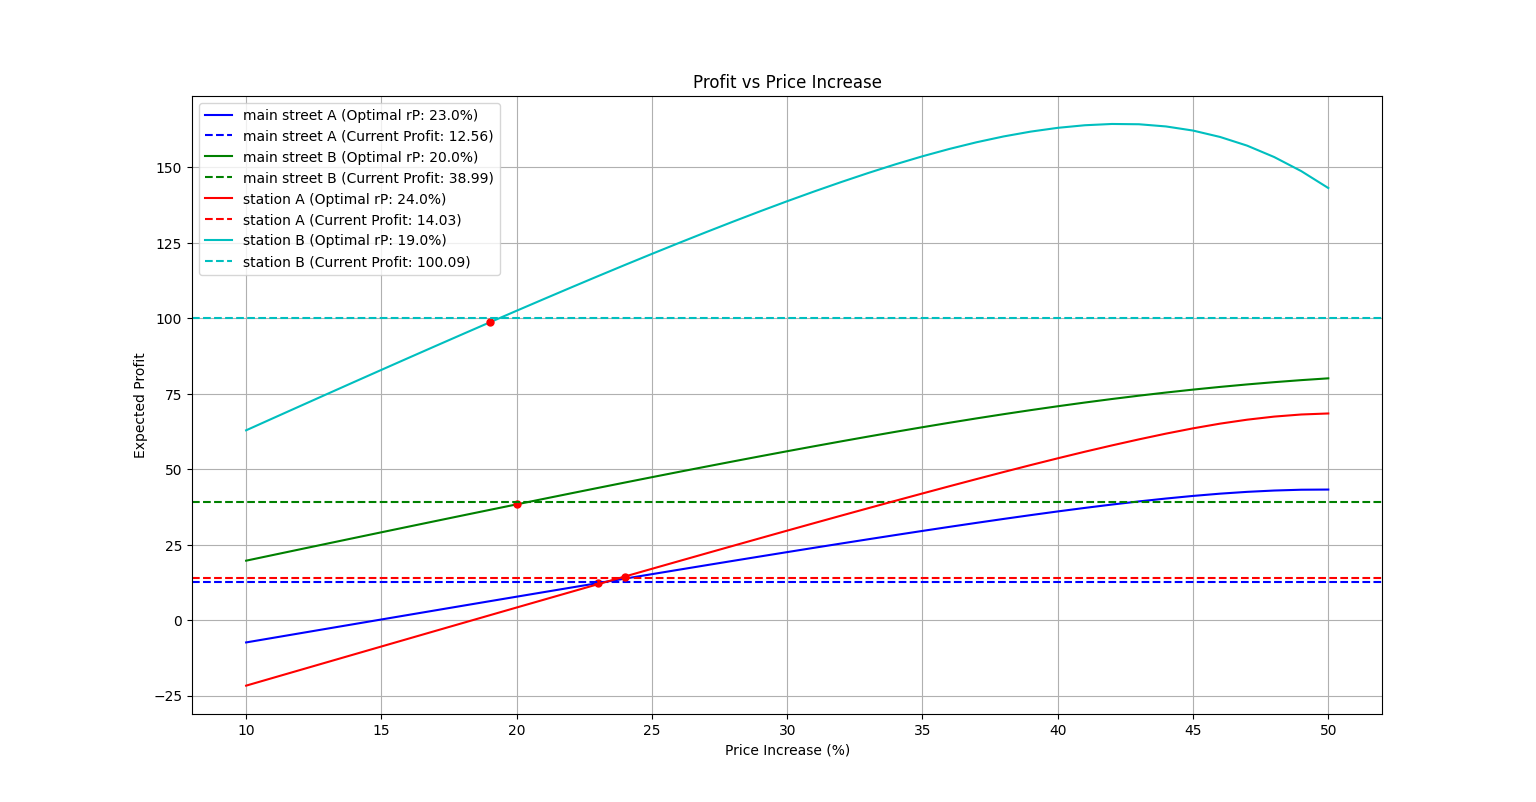
\includegraphics[width=0.85\textwidth]{Static Demand but individual stores.png}
    \caption{Profit vs. Price Increase under Static Demand (Individualized Stores)}
    \label{fig:static}
\end{figure}


The price increases required to maintain current levels of profitability are approximately 23.0\% for \textit{Main Street A}, 21.5\% for \textit{Main Street B}, 25.0\% for \textit{Station A}, and 19.0\% for \textit{Station B}. The graph indicates that beyond these optimal points, profit initially rises due to price increases outpacing the corresponding demand reduction. However, profit subsequently declines, implying that the model prioritizes \textbf{profit stability} over maximization.

\vspace{1em}

Assuming dynamic demand, with individualized store-level analysis, the results are shown in Figure~\ref{fig:dynamic}.

\begin{figure}[H]
    \centering
    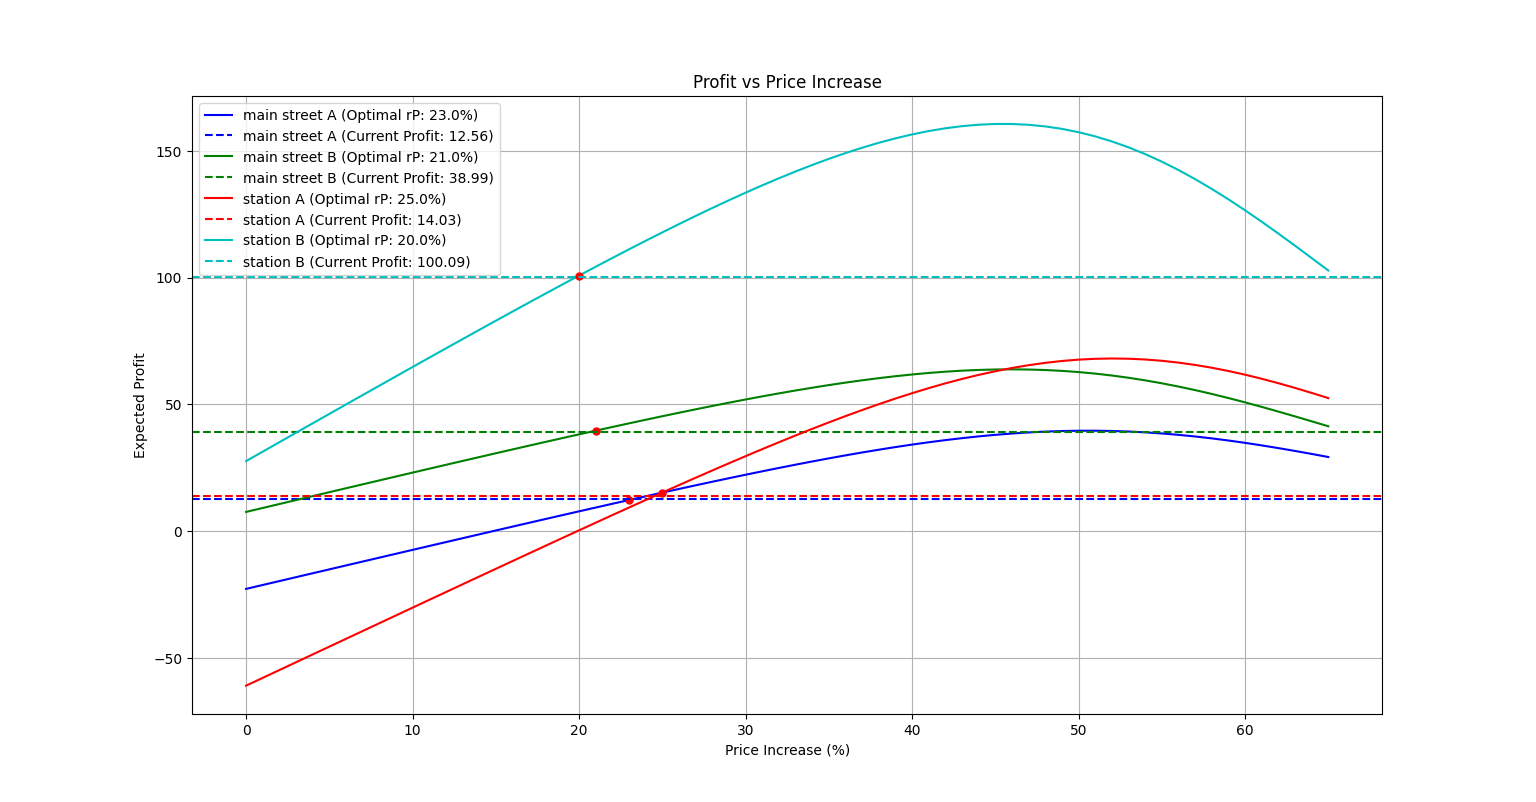
\includegraphics[width=0.85\textwidth]{Dynamic Demand.png}
    \caption{Profit vs. Price Increase under Dynamic Demand (Individualized Stores)}
    \label{fig:dynamic}
\end{figure}

The estimated price increases to maintain current production levels under dynamic demand are approximately 22.5\% for \textit{Main Street A}, 20.8\% for \textit{Main Street B}, 24.3\% for \textit{Station A}, and 18.5\% for \textit{Station B}. Once again, profits rise beyond the optimal price points, as the price increases initially outpace demand reductions, but then decline around 40--60\% due to more significant demand drops. As described in the methodology, optimal order quantities were dynamically adjusted using a nonparametric bootstrap approach. This model again emphasizes profit stability rather than maximization.

As stated in the methodology, the scenario assuming dynamic demand, with individualized store metrics, is the most realistic simulation that was run, and thus the results from Figure~\ref{fig:dynamic} would be the recommendation given to the store owners if they want to maintain current profit levels. The results, as seen, however, do not vary so significantly; this is thought to have happened due to the relatively tame effect a price increase has on demand reduction (26.64\% decrease for a 50\% price increase). Moreover, smaller price increases led to even milder effects:
\begin{itemize}
    \item 2\% increase → 0.05\% demand drop
    \item 10\% increase → 0.4\% demand drop
    \item 20\% increase → 1.54\% demand drop
    \item 30\% increase → 4.49\% demand drop
    \item 40\% increase → 11.67\% demand drop
\end{itemize}

This reinforces the conclusion that moderate price increases can effectively preserve profit levels without significantly harming demand.


\section*{Task 8: Critical Review}
\paragraph{}
During our work with the newsvendor problem, we came across both strengths and weaknesses of the methods introduced during the course, that are worth discussing. Using parametric models, like normal and log-normal distributions, was a convenient solution that let us determine optimal order quantities with relative ease. However, these models heavily rely on distributional assumptions that may not be fully available in reality, due to the distributional uncertainty we are often met with when analyzing real-world datasets. For instance, stores such as Station B, which experience multimodal or very skewed demand, made us question the suitability of classic distribution forms. On the other hand, non-parametric approaches that we introduced through bootstrap methods offered much more flexibility, but at lower sample sizes they became increasingly less reliable, and their estimations were inconsistent. 


Our modeling approach was built on a number of necessary assumptions. We presumed that demand was independent and identically distributed (i.i.d.) over time, and that all values related to cost such as those of production, clearance, and shipping could be expressed as stable average values. These assumptions enabled us to perform a manageable analysis that aligned with theoretical concepts introduced and discussed during the lectures, however they inevitably gloss over the intricate details and difficulties that retail operations face in reality.

For example, demand often varies due to external factors like holidays, economic conditions or even weather changes, none of which we directly took into account and modeled. Similarly, the fixed price-demand relationship we used in Task 7, despite being based on our internal research, operates on the assumption that consumer sensitivity is uniform across different locations and times, which might not exactly be the case in reality.

Despite these limitations, applying both theoretical and empirical models significantly helped our understanding of stochastic inventory management. The difference between parametric and nonparametric methods, which initially could have seemed abstract, became much more understandable as we applied them to real data. We noticed that parametric models work well when the assumed distribution matches the provided data, like in the case of \emph{Main Street A}, but can mislead when the fit is not as clear.

In contrast, nonparametric methods proved to be more robust under uncertain assumptions, although they required careful management of sampling variability. Task 7, in particular, improved our understanding of the relationship between customer behavior and operational decisions. We simulating the impact of price increases on demand, which showed how it influences optimal ordering. We showcased the practical benefit of merging profit modeling with behavioral economics.

Looking ahead, there is plenty of room for improvement. Future research could integrate time-series models to take into account autocorrelation temporal trends in demand, especially for stores that experience seasonal changes. Additionally, incorporating external factors like local events or competitor pricing into our demand model could improve future forecast accuracy.

From a methodological standpoint, considering robust optimization or Bayesian methods might provide alternatives that better address the issues of parameter uncertainty or model misspecification. Lastly, shifting our focus from aggregate demand to considering customer-level differences in price sensitivity would allow for more refined inventory and pricing optimizations, ultimately boosting both customer satisfaction and profitability of the operations.


\vspace*{4cm}
\bibliographystyle{plainnat}
\bibliography{references}
\end{document}